\documentclass{whutmod}
\usepackage{metalogo}
\usepackage{setspace}
\usepackage{subfigure}
\usepackage{caption}
\hypersetup{
colorlinks=true,
linkcolor=black
}
\usepackage{amstext} 
\usepackage{amssymb}
\usepackage{float}
\usepackage{booktabs}
\usepackage{graphicx}
\usepackage[linesnumbered,ruled,lined]{algorithm2e}


\team{1}	% 组号
\membera{阮滨}
\joba{编程}
\memberb{王宇}
\jobb{建模}
\memberc{王家柯}
\jobc{写作}

\title{基于投影寻踪法的黄河水质评价}
\tihao{4} % 题号

\begin{document}
\begin{spacing}{1.2}


\maketitle

\begin{abstract}\setlength{\parskip}{0.3\baselineskip}
	黄河作为宁夏地区的主要供水水源,其水生态保护具有重要意义。本文通过\textbf{经验正交函数分解}提取了水污染
	的时空规律,运用\textbf{模糊综合评价法}对断面水质进行综合评级,最后使用\textbf{实数编码加速的遗传算法}求解\textbf{投影寻
	踪评价模型},得到了各断面处黄河水生态系统评分。

	针对问题一,从水质的\textbf{综合污染情况和单一指标超标情况}分别对黄河宁夏河段水质进行分析。在综合污染
	情况的分析中,本文在国标规定的以最劣指标确定水质等级的基础之上,通过\textbf{模糊综合评价}对当前水质的整
	体情况以及与目标水质之间的差距进行补充说明;在各指标超标情况的分析中,本文以目标水质对应各指标
	的下限作为阈值,统计了水污染指标超标的种类以及次数。发现虽然较多断面水质未达国家标准,但实际上
	综合水质情况较为乐观,仅有个别指标不达要求,后续可以采取针对性措施的对水质进行治理。
	
	针对问题二,本文通过\textbf{经验正交函数分解法}对黄河宁夏河段水质的时空规律进行分析。考虑到\textbf{枯水期和丰
	水期}黄河流量的较大差异,本文首先将数据按此标准进行划分,基于\textbf{经验正交函数分解法}分别对两个时期
	的\textbf{时间模态和空间模态}进行提取,通过\textbf{Mann-Kandell检验}得到各水质指标在时间维度的趋势,并运用\textbf{Nor
	th检验}验证了经验正交函数分解法的可信度。从时间维度分析发现从1月到8月,\textbf{氨氮浓度、生化需氧量等
	四个指标}呈增加趋势,而\textbf{铜和硫化物}具有减少趋势;而在空间维度发现整体水质由上游到下游逐渐变好,
	初步分析与国家对于出境水质的监管和处罚规定有关。
	
	针对问题三,综合考虑黄河水生态中的各要素,构建指标体系,并建立了\textbf{投影寻踪模型}进行综合评级。
	首先通过查阅资料,\textbf{从水质、水量以及人类开发等六个维度出发},选择了包括\textbf{河岸基质类型、径流变化率
	等十六个指标},并建立\textbf{投影寻踪模型}对各断面的水生态进行综合评分。通过\textbf{实数编码加速的遗传算法}对
	模型进行求解,得到了相应的得分。之后将各指标的等级阈值代入到投影寻踪评价模型中,得到了相应
	的分数阈值,最后得到了黄河水生态综合状况所属的等级。结果发现存在较多的水生态整体情况不达标
	,仍有较大的提升空间。
	
	本文的优点包括:1.通过经验正交函数分解法得到了水质指标的时空模态,既能分别获取水污染在
	时间和空间上的规律,又能分析任意两断面指标变化的关联性。2.采用投影寻踪模型对黄河宁夏河
	段水生态坏境的整体情况进行评价,其结果为连续评分与离散等级相结合,更为科学合理。

		\keywords{
			水质评价\quad
			模糊综合评价\quad
			正交经验分解 \quad
			投影寻踪\quad
			实数编码加速的遗传算法



		}
\end{abstract}


\tableofcontents
\thispagestyle{empty}

\newpage
\setcounter{page}{1}

\section{问题重述}



	\subsection{问题背景}
	黄河作为中华民族的“母亲河”,在宁夏段由于长期接纳工业废水、生活污水和农田退水,使得宁夏全区地面水环境
	已受到不同程度的污染。作为宁夏最重要的地表水资源,如何评价分析黄河的水质情况对黄河的治理十分必要。

\begin{figure}[H]
		\centering
		
\includegraphics[width=.6\textwidth]{背景.png}
		\label{上下车人数示意图}
		\caption{水污染治理}
\end{figure}


\subsection{问题重述}

	问题一:结合附件中的内容,通过处理文中的数据得出结论分析黄河宁夏段某河段上的水环境污染现况。

	问题二:结合数据,建立数学模型,得到黄河某段水污染的现状规律。

	问题三:通过提出一个合理的评价体系,建立一个评价模型评价黄河水环境、水生态

\section{模型的假设}

\begin{itemize}
		\item 采样断面点位置设置合理,数据具有有效性;
		\item 一周内采样数据数值稳定不变;
		\item 选取指标能够有效反应水质。
		
\end{itemize}






	\section{符号说明}
	\begin{center}
		\begin{tabular}{cc}
			\\\toprule[1.5pt]
			\makebox[0.3\textwidth][c]{符号} & \makebox[0.4\textwidth][c]{意义} \\ \hline
			$Y$                       & 隶属度            \\
			$w_i$                            & 权重                  \\
			$\lambda $                           & 特征                 \\
			$x_{(i,j)}$                       & 样板集                     \\
			$R_{zy}$                         & 标准差                   \\
			\bottomrule[1.5pt]
		\end{tabular}
	\end{center}
	注:其他未列出的符号以第一次出现时的解释为准。

	\clearpage




\section{问题一的模型建立与求解}

\subsection{问题分析}

根据《地表水环境质量标准GB3838-2002》的相关要求,水质应该按照所有检测指标中最差的等级进行评级。此
方案具有合理性,因为任何一个成分超标都会导致水源无法正常使用。

但是此评级方案无法区分同一类水质中的差别,且很可能仅因一个成分超标就导致评级结果远超目标值,无法客观
反映当前水质与目标水质之间的距离$^{[1]}$。故本文拟通过模糊综合评价法得到水质综合等级的对原本依照国标确定的水质等级进行补充说明$^{[2]}$。

此外,本文拟通过对各断面水质的单一成分超标情况进行统计,分析黄河主要容纳的污染成分。
\begin{figure}[H]
	\centering
	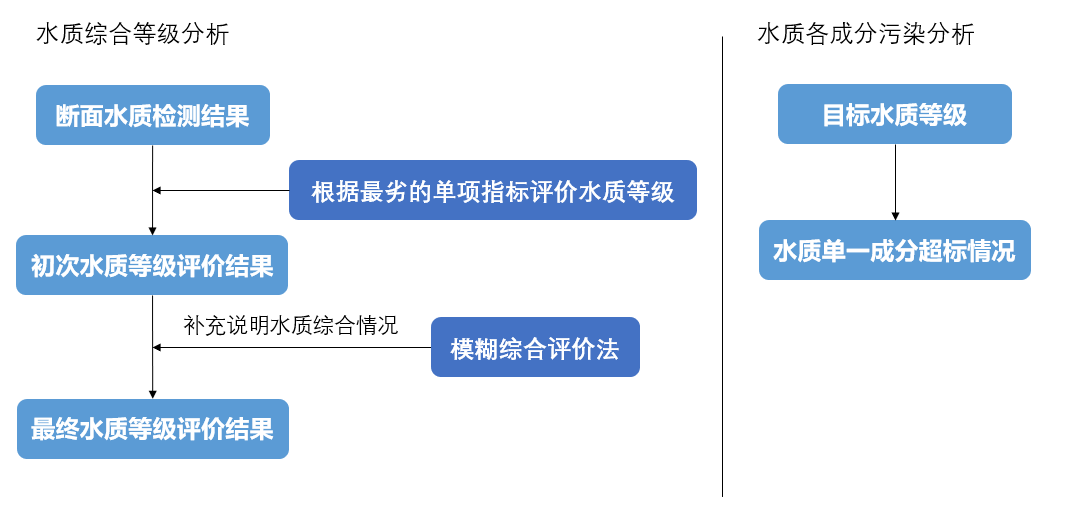
\includegraphics[width=.8\textwidth]{问题一思路图.png}
	\label{问题一思路图}
	\caption{问题一思路图}
\end{figure}




\subsection{数据预处理}
通过观察附件中的所给数据,可以发现A站点在七月份和八月份的所有数据都为-1,属于异常数据。
根据备注中的说明,这些异常数据的产生是因为监测点被堵塞,故本文选择剔除这些数据。

此外,通过查阅《地表水环境质量标准GB3838-2002》,发现在水质检测的过程中,已经进行了重复实验
保证结果的可靠性,故本文对附件中标红的超标数据不做额外处理。



\subsection{模糊数学综合评价模型}

模糊数学综合评价法的基础理论是隶属度理论,即用属于分别五类水质标准的程度大小去代替属于或不属于该种标准,用隶属度对受
多种条件限制的事物作出总的评价。以下是具体步骤:
~\\
\textbf{1)建立综合评价因素集}
	 
因素集是有影响评价水质的因素组成的集合,通常用$U=(U_1,U_2,U_3,...,U_m)$,其中m是评价因素的个数。本文选择21个评价因素,
即$U=(U_1,U_2,U_3,...,U_21)$,其中分别表示为每种重金属的含量。
~\\
\textbf{2)建立综合评价的评价集}

评价集是由各评价对象可能获得的结果所组成的集合,通常用V表示,$V=(V_1,V_2,V_3,...,V_n)$,其中n表示评价集的个数。水质
评价按功能高低共有I~V五类级别,所以,本文设定评价集为$V=(V_1,V_2,V_3,V_4,V_5)$。
~\\
\textbf{3)计算隶属度}

将某种事物属于某种标准的程度称为隶属度。水体水质好坏的程度界定较为模糊, 可以用隶属函
数来刻画模糊的水质等级边界。隶属度可以用隶属函数表示:
\begin{equation}
	\label{2}
	\begin{split}
    Y=\frac{X-X_0}{X_1-X_0} \mbox{或} \frac{X_1-X}{X_1-X_0},
	\end{split}
\end{equation}
式中,Y为隶属度;X为实际监测值;$X_0$、$X_1$为两相邻水质标准所对应的值。
~\\
\textbf{4)定各因子在综合评价中的权重}

权重公式为$W_i=\frac{C_i}{S_i}$
式中,$W_i$
\begin{equation}
	\label{2}
	\begin{split}
     W_i=\frac{C_i}{S_i}.
	\end{split}
\end{equation}
式中,$W_i$为评价参数权重;$C_i$为i项检测指标浓度的实测值;$S_i$为i项检测指标的标准浓度平均值。
~\\
\textbf{5)模糊矩阵的复合运算}

   将权重行列式与隶属度矩阵进行综合运算, 得到模糊综合评价向量, 根据最大隶属原则可知, 综
合评价向量中的最大隶属度所对应的评价等级即为模糊评价的水质等级。

\subsection{模型求解}
通过python编程进行求解,本文依据国标对每一个类型的水质进行模糊综合评价
将附件中五类中的每一类水再细分为A、B、C、D、E(品质由高到低)
五个类别。如图\ref{水质等级说明}所示方式进行编码。

\begin{figure}[H]
	\centering
	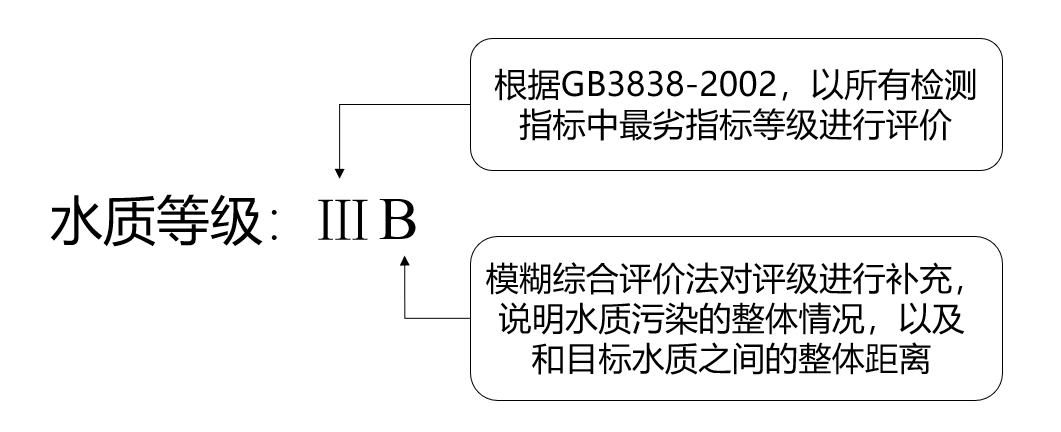
\includegraphics[width=.8\textwidth]{水质等级说明.png}
	\label{水质等级说明}
	\caption{水质等级说明}
\end{figure}


% Table generated by Excel2LaTeX from sheet 'Sheet2'
\begin{table}[htbp]
	\centering
	\caption{各月份各界面水质细分表}
	  \begin{tabular}{ccccccccc}\toprule[1.5pt]
		  & 1月   & 2月   & 3月   & 4月   & 5月   & 6月   & 7月   & 8月 \\ \hline
		  A   & VE  & VE  & VE  & IVD  & IVC  & IVC  & \textbackslash{} & \textbackslash{} \\
		  B   & VE  & VD  & VE  & VC  & VB  & VC  & IVA  & IIIA \\
		  C   & VE  & IVD  & IVD  & IIIB  & VE  & IVC  & IIIA  & IIIA \\
		  D   & IIIA  & IIIA  & VE  & IIIB  & IVC  & IIIC  & IIIA  & IIIA \\
		  E   & IIB  & IIIC  & IIIC  & IIIA  & VD  & IVB  & VE  & IIIA\\ \bottomrule[1.5pt]
	  \end{tabular}%
	\label{xifen}%
  \end{table}%
  
计算结果如表\ref{xifen}所示,其为利用模糊综合评价对国家标准水质等级补充后形成的新的水质检
验结果表,例如:E站点中六月的水质情况为Ⅳ类水中的B类品质,其中V类表示此次检测中,水质各指标最差的
等级为Ⅳ类;而B则表示其水质综合情况较好,大部分指标都能够满足要求。综合来看,虽然最差的指标属于Ⅳ类
,但是该水质综合情况良好,具有较大的提升潜力。

\subsection{结果分析}
\subsubsection{综合污染情况分析}
以下图\ref{水质分布示意图}是水质分布图,图\ref{超标次数频数统计图}是贡献率最大的几种
污染物的超标次数频数统计图。


\begin{figure}[H]
	\centering
	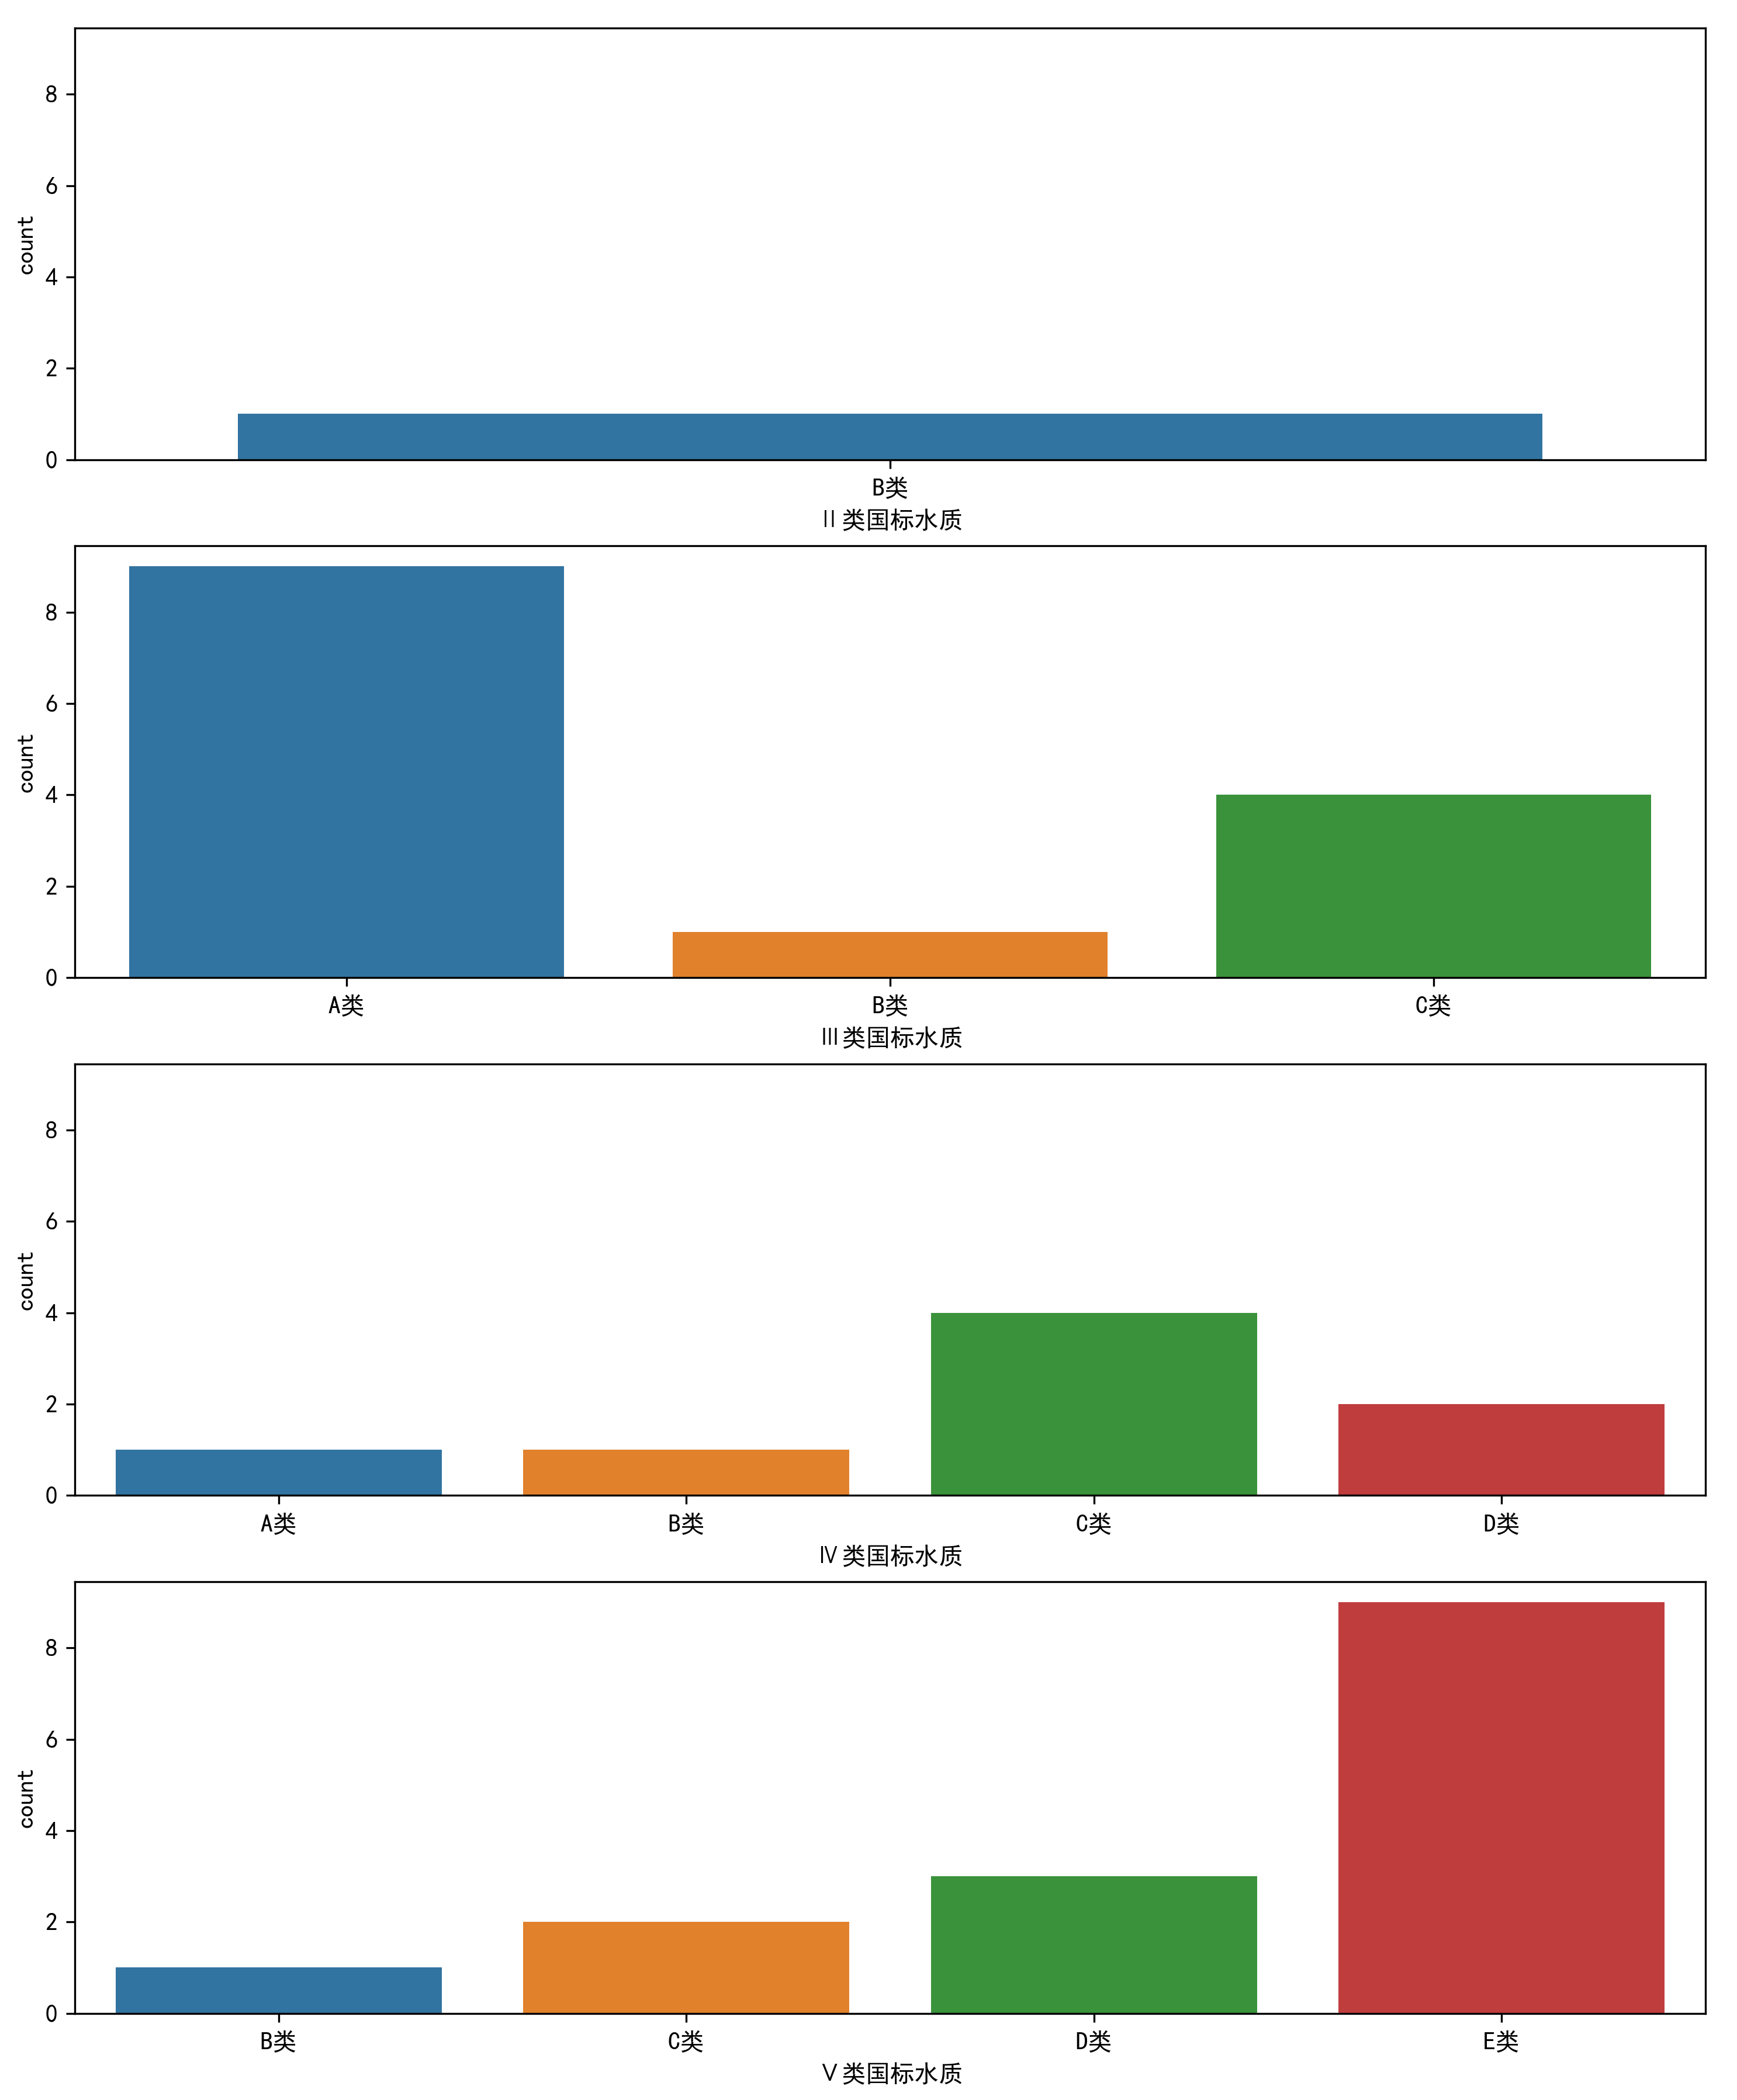
\includegraphics[width=.8\textwidth]{细分.png}
	\caption{水质分布示意图}
	\label{水质分布示意图}
\end{figure}

从图中可以看出,宁夏水质情况处于II-V类水质,大部分为IV、V类水质。与宁夏河段Ⅲ类目标水质进行对比
仍有大部分水质处于不达标的状态,但是观察每个等级中模糊综合评价的结果,发现尤其是Ⅲ类和Ⅳ类水,
水质的综合情况往往比最差指标所属的等级要好,故说明这些水往往是由于个别指标严重超标导致的水质不合格
需要针对性的进行管控;而对于Ⅴ类水,其模糊综合评价的结果也大多数属于E类,说明该水质的整体情况也
不容乐观,需要进行全方面的管控。

\subsubsection{单一指标超标情况分析}

\begin{figure}[H]
	\centering
	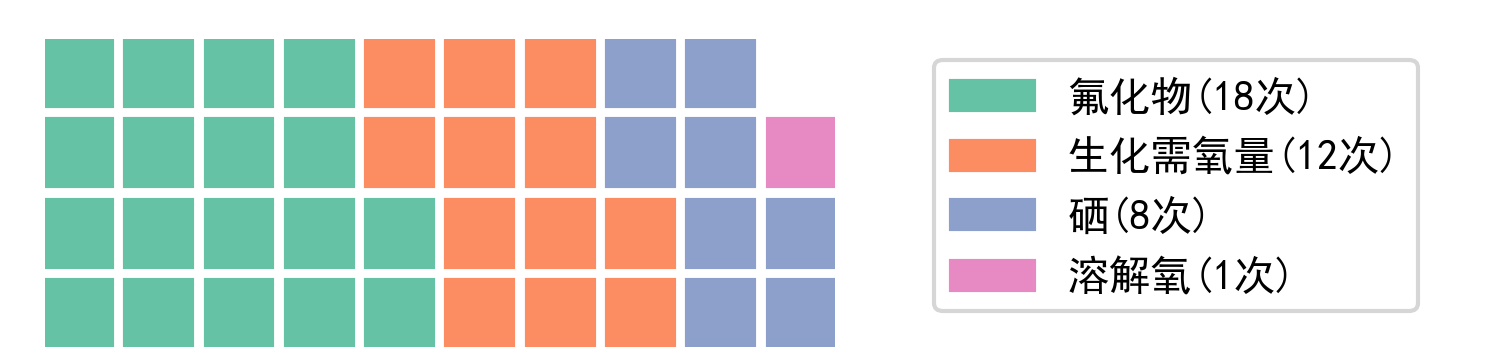
\includegraphics[width=.9\textwidth]{超标次数频数统计图.png}
	\caption{超标次数频数统计图}
	\label{超标次数频数统计图}
\end{figure}

图中为单污染分析下的每一种主要污染物的污染次数,可以发现黄河宁夏河段的污染物种类
比较有限,仅有生化需氧量、溶解氧、硒以及氟化物四类污染物超标。其中主要污染的指标为氟化物和生化需氧量
,其对水质污染的贡献率高达46.2\%,而生化需氧量的贡献率也达到了30.8\%。
说明了黄河宁夏段上游受到含有氟化物的工业废水污染较为严重,后续需要针对分析成因,重点排查相关企业。

\section{问题二模型的建立与求解}



\subsection{问题分析}

黄河具有着明显的枯水期和丰水期,两个时间段内的流量具有明显差异,对污染物的稀释能力也不相同。刘姜艳在《黄
河流域水污染现状分析及控制》$^{[3]}$中指出黄河的枯水期为10月至次年6月,而丰水期则为7月至9月。本文拟将附件中八个
月的断面水质检测数据按照上述方法分成两组分别进行研究。

为提取水环境污染的规律,本文从时间和空间两个角度进行考虑。故拟通过经验正交函数分解法对样本进行分析,分
别得到时间和空间模态,并对时间模态进行趋势检验。

\begin{figure}[H]
	\centering
	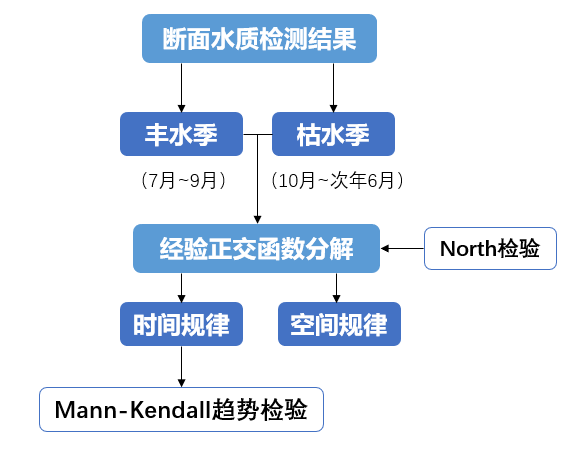
\includegraphics[width=.8\textwidth]{问题二思路图.png}
	\label{问题二思路图}
	\caption{问题二思路图}
\end{figure}



\subsection{建立经验正交函数分解模型(EOF)}

为获取黄河宁夏段各前面水质情况的时空分布,应采取模型将水质情况分解至时间维度和
空间维度。本文认为水质情况分别在时间维度和空间维度都具有相应的模态。因此本文选用
正交经验分解模型,拟分别提取出经典的时空模态。另外考虑到数据的分布不一定为正态分布
,故采用Mann-Kendall趋势检验。此方法不依赖数据的分布,且能都避免异常数据干扰。以下是模型建立的具体步骤:
~\\
\textbf{1)数据预处理}
选定要分析的水质数据,进行数据的预处理,通常处理成距平的形式得到一个数据矩阵$X_{m\times n}$

~\\
\textbf{2)得到方阵}
计算$X$与其转直矩阵$X$的交叉积,得到方阵
 
\begin{equation}\label{eq:dirchlet}
      C_{m\times m}=\frac{1}{n}X\times X^T .
\end{equation}

如果$X$是已经处理成距平的话,则称$C$为协方差阵;如果$X$已经标准化(即$C$中每一行数据的平均值为0标准差为11
)则称为相关系数矩阵。

~\\
\textbf{3)计算特征根和特征向量}
计算方阵$C$的特征根$ (\lambda_{1} ,\lambda_{2} ,...,\lambda_{m}) $和特征向量$V_{m\times m}$
,二者满足

\begin{equation}\label{eq:dirchlet}
	C_{m\times m}\times V_{m\times m}=V_{m\times m}\times E_{m\times m},
\end{equation}
其中$E$是$m\times m$维对角阵,即
$$E=\begin{bmatrix}
	\lambda_{1} & 0 & \cdots & 0\\
	 0 & \lambda_{2}& \cdots & 0\\
	 \vdots &\vdots & \ddots &\vdots \\
	 0 & 0 & \cdots & \lambda_{m}\\
\end{bmatrix}$$

一般将特征根$\lambda$按从大到小排列。因为数据$X$是真实的观测值,所以$\lambda$应该大于等于0.每一个非0的特征根
对应一列特征向量值,也称EOF。


~\\
\textbf{4)计算主成分}
将EOF投影到原始资料矩阵上,就得到所有空间特征向量对应的时间系数(即主成分),即

\begin{equation}\label{eq:dirchlet}
     PC_{m\times n}=V_{m\times m}^T \times X_{m\times n},
\end{equation}
其中PC中的每一行数据就是对应每个特征向量的时间系数。

~\\
\textbf{5)计算贡献率}
矩阵 $X$ 的方差大小可以简单的用特征根的大小来表示。 $\lambda $越高说明对应的模态越重要,对总方差的
贡献越大。第$k$个模态对总的方差解释率为
\begin{equation}\label{eq:dirchlet}
	\frac{\lambda_k}{\sum_{i=1}^m\lambda_i}\times100\%.
\end{equation}

~\\
\textbf{6)显著性检验}
实际资料分析中得到的空间模态是否是随机的,需要进行统计检验。North等(1982)的研究提出
,在95\%置信度水平下的特征根的误差

\begin{equation}\label{eq:dirchlet}
	\delta \lambda = \lambda \sqrt{\frac{2}{N^*}},
\end{equation}
其中$\lambda$是特征根,$N^*$是数据的有效自由度。将$\lambda$按顺序依次检查,标上误差范围。如果前后两个$\lambda$
之间误差范围有重叠,则没有通过显著性检验。



\subsubsection{Manner-Kendall(M-K)非参数检验法}

Manner-Kendall(M-K)非参数检验法常用于分析降水、径流、气温等要素时间序列的变化趋势。本文采用此方法
对1到6月枯水期的数据进行M-k趋势检验。

设有n个样本量的时间序列$x_{1},x_{2},\cdots,x_{n}$,对于所有$k,j \le n $,且$x_k$和$x_j$的分布是不懂得
,计算检验统计量$s$,公式如下:

\begin{equation}\label{eq:dirchlet}
	S=\sum_{k=1}^{n-1}\sum_{j=k+1}^{n} Sgn(x_j-x_k),
\end{equation}
其中

\begin{equation}\label{eq:dirchlet}
	Sgn(x_j-x_k)=\begin{bmatrix}
		+1(x_j-x_k)>0,\\
		0(x_j-x)=0,\\
		-1(x_j-x_k)<0;
	\end{bmatrix}
\end{equation}
s为正态分布,均值为0,方差$var(s)=n(n-1)(2n+5)/18$。当$n>10$时,标准正态统计变量通过下式计算:
\begin{equation}\label{eq:dirchlet}
	Z=\begin{bmatrix}
		\frac{S-1}{\sqrt{var(S)}}>0,\\
		\frac{S+1}{\sqrt{var(S)}}<0.\\
	\end{bmatrix}
\end{equation}






\subsection{模型求解}	
利用matlab进行求解,可以得到各个污染物的变化趋势,如下表\ref{趋势},图\ref{变化趋势}为
变化明显的污染物变化趋势大小关系图。图\ref{时间系数}是部分污染物的时间系数变化。


\begin{figure}[H]
	\centering
	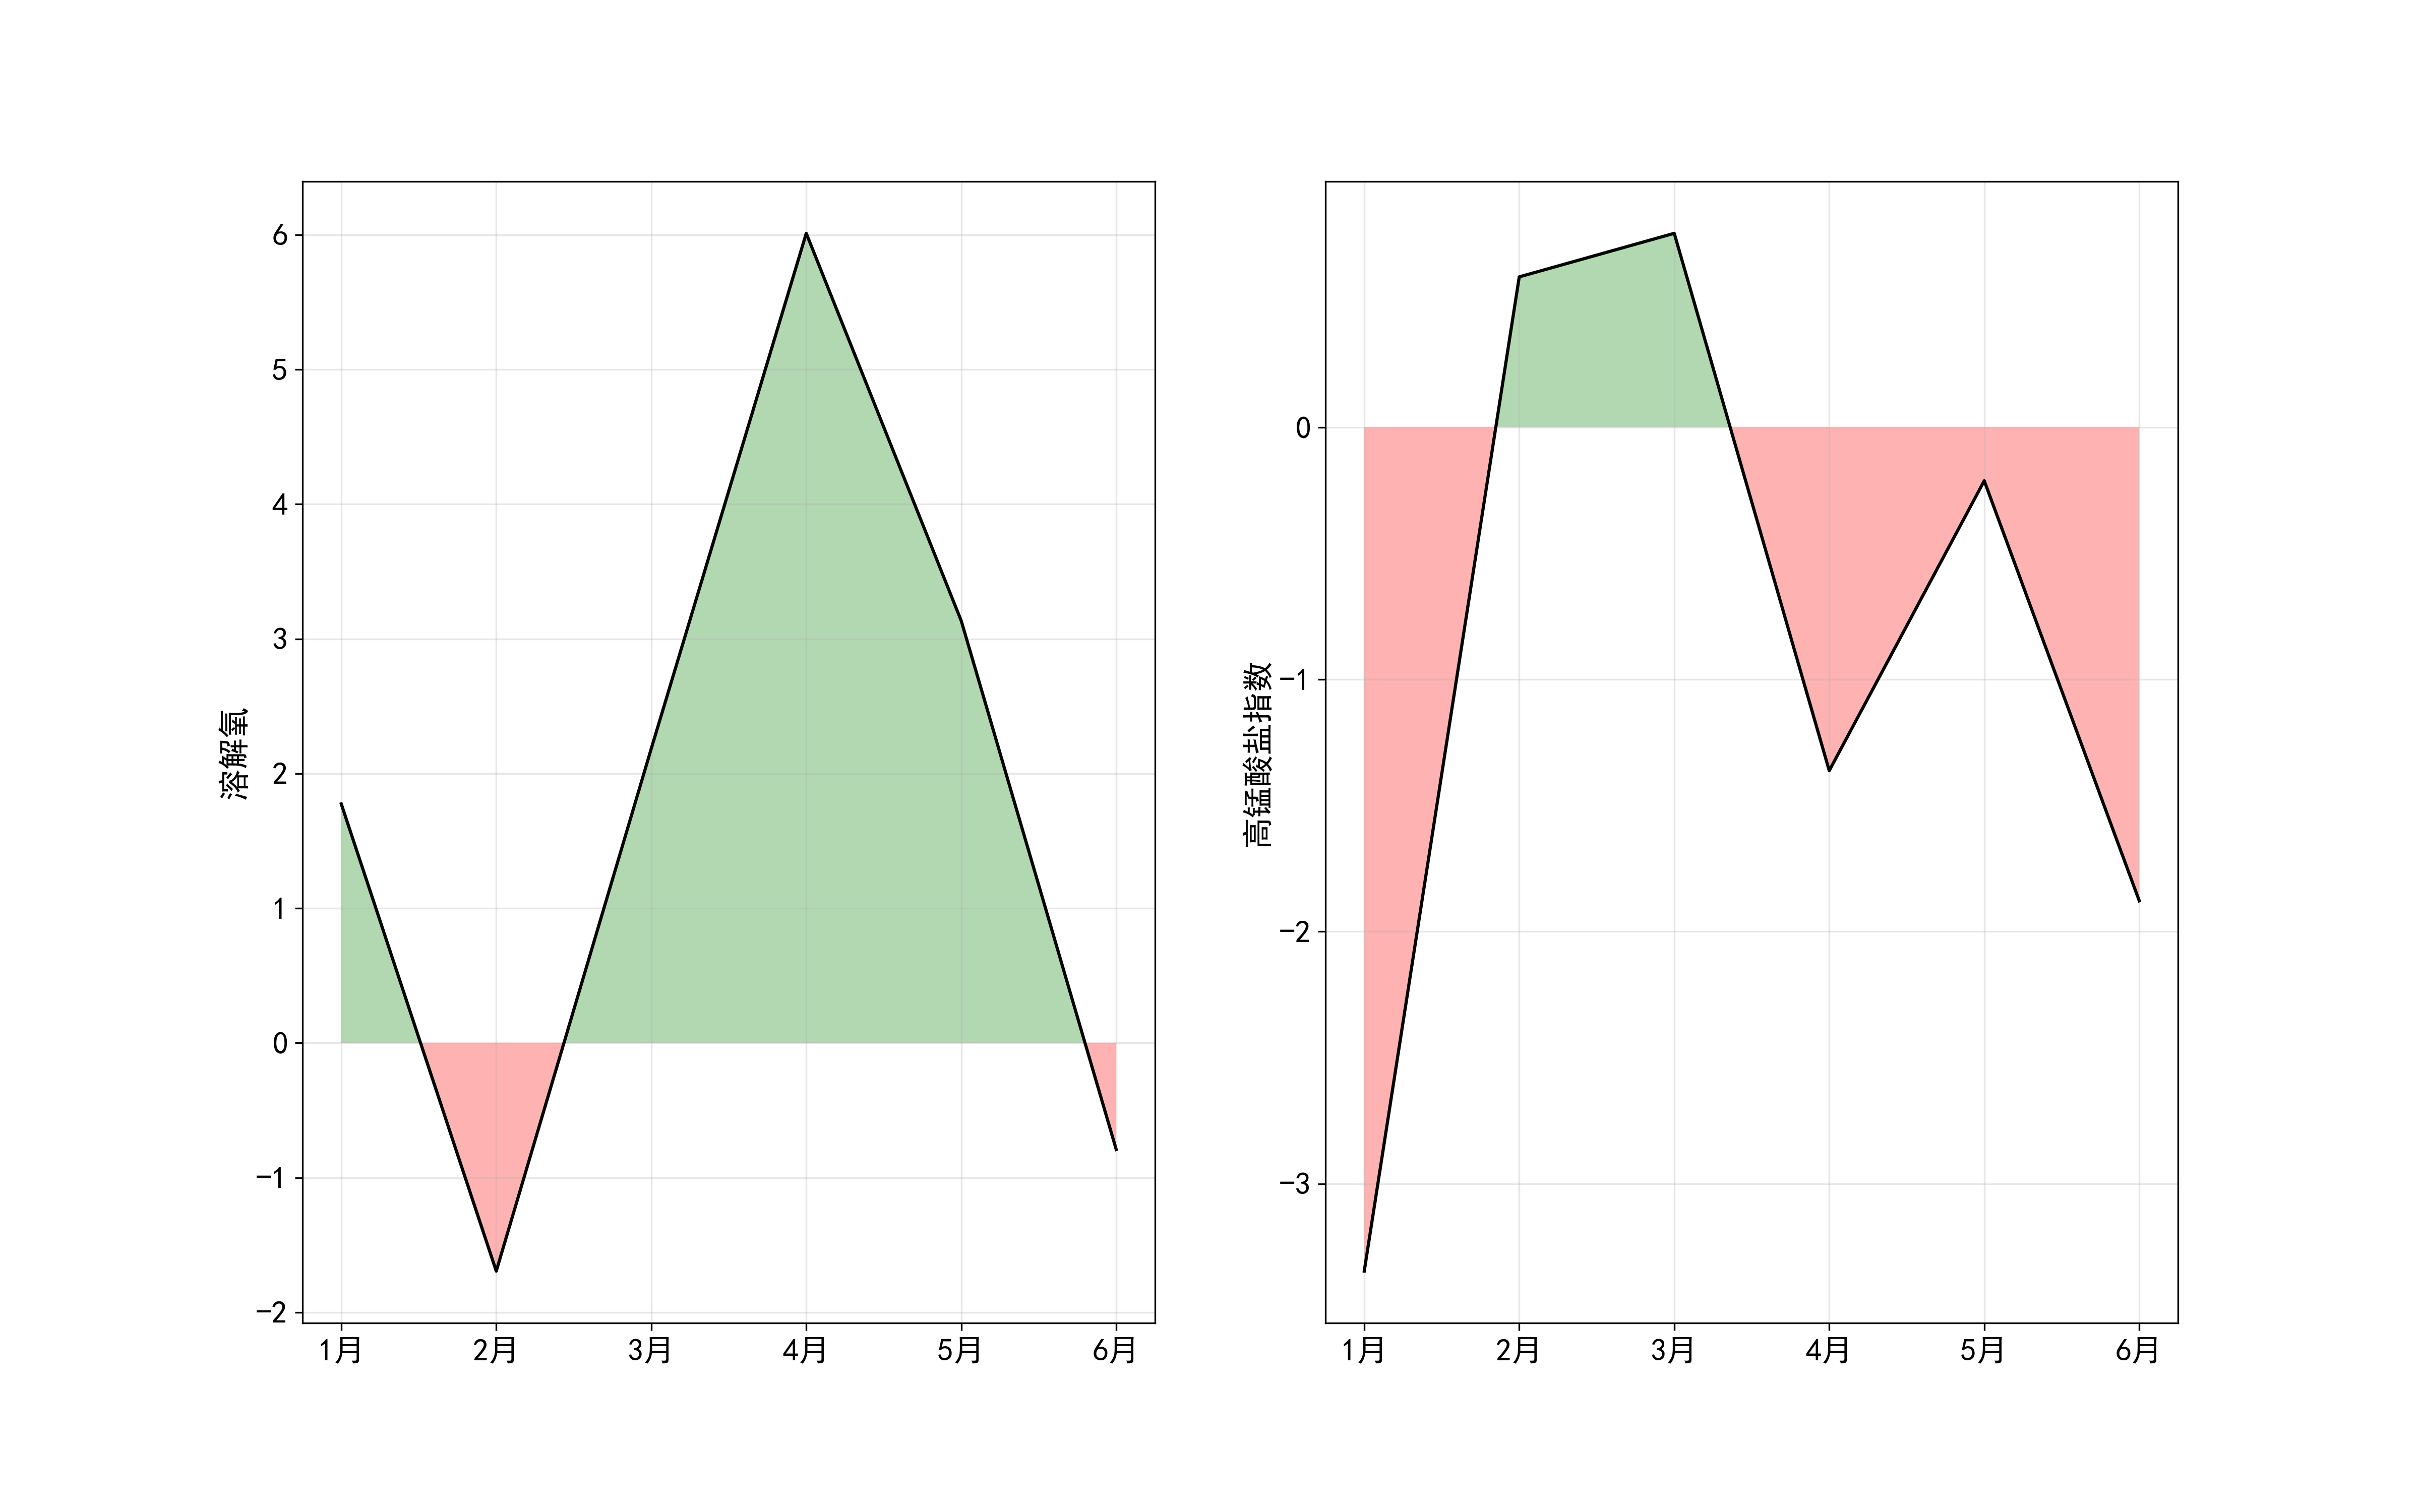
\includegraphics[width=.8\textwidth]{时间系数.png}
	\caption{时间系数趋势图}
	\label{时间系数}
\end{figure}

图\ref{时间系数}为部分污染物的时间模态图,图中可以分别看出溶氧率和高猛酸盐污
染物污染物时间上的变化趋势。其中模态的正负表示各断面变化过程中的正负相关性,以图7(a)为例,当1月份
增加一个单位时,根据统计学意义,模态同为正的3月、4月、5月都会按照一定的比例增加,而2月和6月会按照
一定比例减少。

\begin{figure}[htbp]\centering                                                          %居中
	\subfigure[溶解氧]{                    %第一张子图
	\begin{minipage}{7cm}\centering                                                          %子图居中
		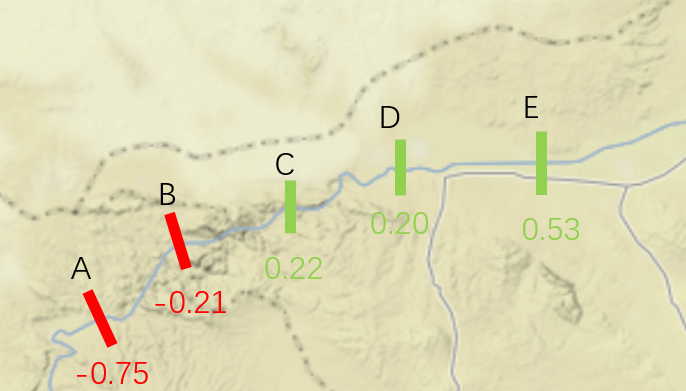
\includegraphics[scale=0.3]{溶解氧}               %以pic.jpg的0.5倍大小输出
	\end{minipage}}
	\subfigure[高锰酸盐指数]{                    %第二张子图
	\begin{minipage}{7cm}
		\centering                                                          %子图居中
		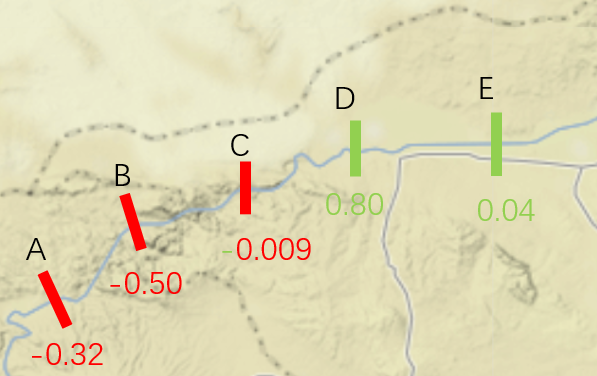
\includegraphics[scale=0.3]{高锰酸盐指数}                %以pic.jpg的0.5倍大小输出
	\end{minipage}}       
	\caption{空间趋势图} %                                              %图片引用标记
	\label{空间趋势}
\end{figure}

图\ref{空间趋势}为部分污染物的空间系数图,图中可以分别看出溶氧率和高猛酸盐污染物在各断面处的情况。
模态正负的含义与上文中时间模态正负的含义相同。从图中不难看出,黄河宁夏河段上游污染情况与下游污染情况
具有明显的差异性,且不难看出下游的污染情况远比上游要轻。

\begin{table}[H]
	\centering
	\caption{污染物变化趋势}\footnotesize
	\begin{tabular}{cccc}\toprule[1.5pt]
		\makebox[0.3\textwidth][c]{污染物} & \makebox[0.4\textwidth][c]{变化趋势} \\ \hline
		生化需氧量 & 增加 \\
		氨氮  & 增加 \\
		铜   & 减少 \\
		砷   & 增加 \\
		六价铬 & 增加 \\
		硫化物 & 减少 \\
		其污染物&无明显趋势\\\bottomrule[1.5pt]	
	 \end{tabular}%
	\label{趋势}%
\end{table}%



\begin{figure}[H]
	\centering
	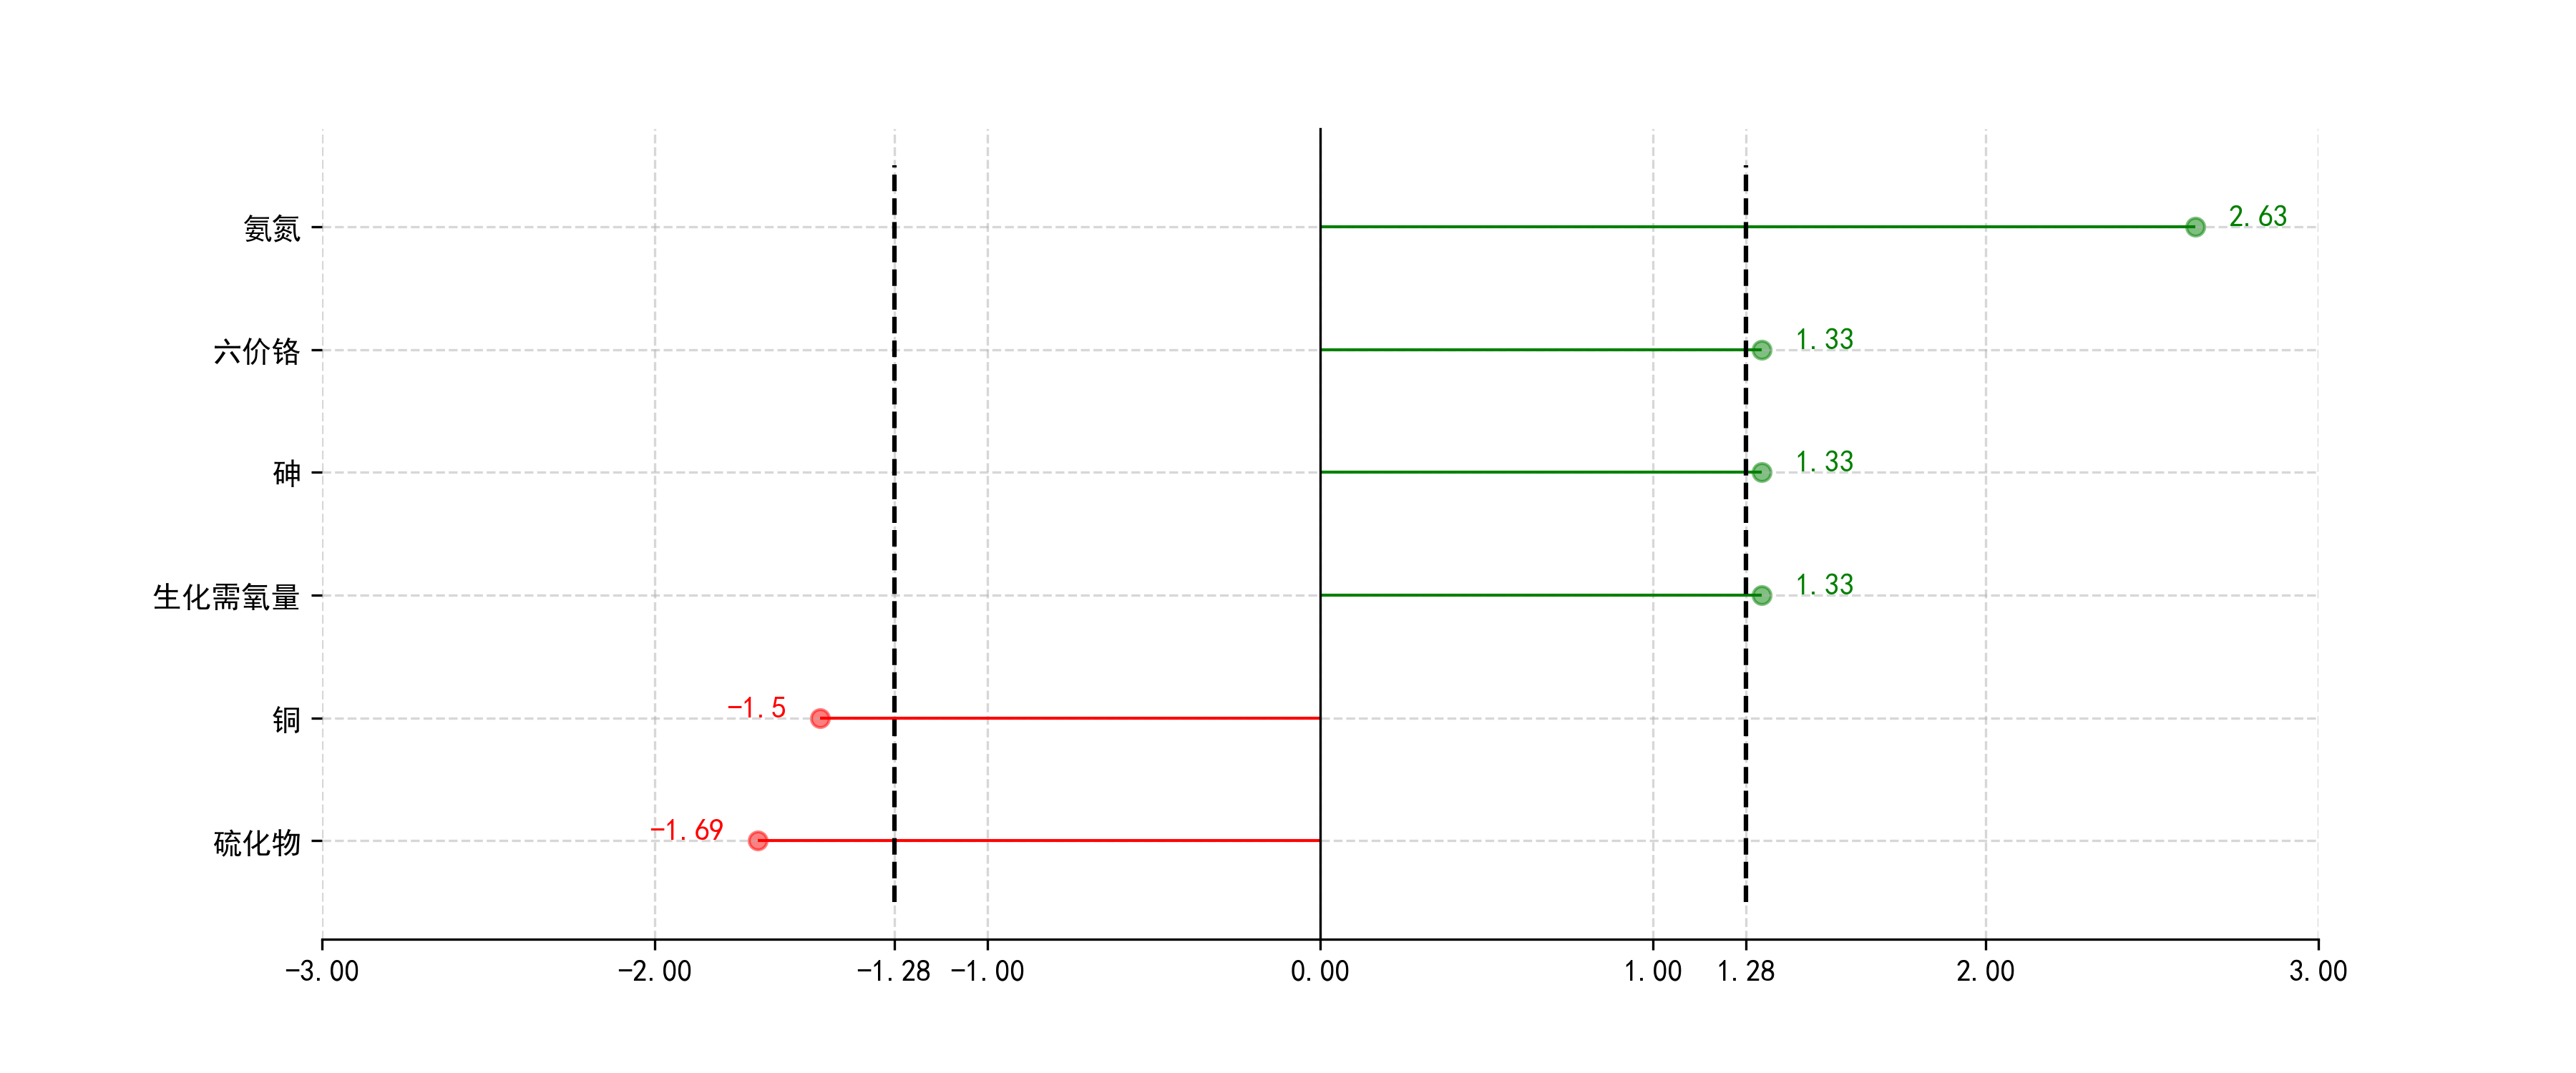
\includegraphics[width=.8\textwidth]{mk检验.png}
	\caption{污染物趋势分布图}
	\label{变化趋势}
\end{figure}

通过图片和表格可以看出,在未来一段时间里氨氮、六价铬、砷、生化需氧量这些污染物浓度有增加趋势,其中
氨氮浓度增大趋势最明显,而铜含量和硫化物则有明显的减少趋势。因此具有增加趋势的污染物需要特别注意。


\subsection{模型检验及结果分析}

\subsubsection{North检验}

为了确定各个模块之间是否相互独立,North检验是最简单也是必须要做的检验。

North检验,是计算特征值误差范围来进行显著性检验。特征值$\lambda$的误差范围
\begin{equation}\label{eq:dirchlet}
     e_j=\lambda_j(\frac{2}{n})^{\frac{1}{2}}
\end{equation}
其中$n$为样本量,当相邻特征值$\lambda_j+1$满足$$\lambda_{j+1}-\lambda_j\ge e_j$$时,认为
这两个特征值对应的经验正交函数是有价值的信号。下表是North检验结果:

\begin{table}[H]
	\centering
	\caption{污染物变化趋势}\small
	\begin{tabular}{cccc}\toprule[1.5pt]
		\makebox[0.3\textwidth][c]{污染物种类} & \makebox[0.4\textwidth][c]{North检验结果} \\ \hline
		高锰酸盐指数 & 12.0249>11.1121 \\
		生化需氧量 & 40.5699>30.8463 \\
		氨氮  & 14.8622>10.1053 \\
		石油类 & 0.0004>0.000252982 \\
		挥发酚 & 1.6e-08>1.01193e-08 \\
		铅   & 5.53667e-05>7.22518e-05 \\
		... & ... \\
		总磷  & 0.0586599>0.063928 \\
		铜   & 0.0001944>0.000122949 \\
		硒   & 1.5552e-05>9.83595e-06 \\
		砷   & 1.23709e-05>9.75207e-06 \\
		六价铬 & 1.25621e-05>5.47598e-05 \\
		阴离子表面活性剂 & 0.008>0.00505964 \\
		硫化物 & 0.000341383>0.000237382 \\
		\bottomrule[1.5pt]	
	 \end{tabular}%
	\label{趋势}%
\end{table}%

通过North检验,可以发现每一个污染物指标都能通过检验,因此可以说明每一个模块的数据都有价值,此模型可以较为
成功的反应实际问题。

\subsubsection{结果分析}

通过正交经验分解(EOF),分别得到了污染物变化的时间模态和空间模态。从空间维度上来说,污染物的分布情况
与上下游之间具有明显的相关性,具体反映在污染情况上则为上游污染更为严重,而下游污染较轻。经过查阅
《中华人民共和国水污染防治法》,发现对于各省出境的水质具有严格要求,不达标则会受到严重的出发,
因此政府可能着重于管理出境河段的污染。因此很有必要完善相关的法律法规,使得全河段的污染情况都得到
严格的管控。

对时间模态经过M-K趋势检验后,本文得到了几种污染物未来的变换趋势,基于此类趋势
可以检验当地污染排放的种类。通过查阅相关资料,发现生化、化工工厂的废水均含有氨氮、六价铬、砷等
污染物,因此建议宁夏有关部门重点排查相关企业,做好排放前的污水治理工作,以此减少黄河污染程度。




\section{问题三模型建立与求解}


\subsection{问题分析}
为建立评价黄河水生态的评价模型,首先需要构建合理的指标体系。在众多学者对生态评价的研究中,都将问题转
化为生态承载能力的评价$^{[4]\sim[6]}$,故指标体系中不仅需要考虑到黄河水质,还需要考虑到人类开发程度、
黄河河岸及其周边环境等。

目前,国内大量学者对黄河流域的相关指标进行了探索。田野在《黄河内蒙古段河流健康评价》中提出了对河床、河
岸等物理结构的相关指标,张丽洁在《黄河流域水资源评价研究》中提出了水质、水量等维度的指标。本文在上文中
选取了具有代表性的6个一级指标以及16个二级指标。

此外,本文拟通过实数编码加速的投影寻踪法$^{[7]}$对各指标进行赋权,得到黄河水生态的最终评价结果。并且,本文将权
重与上述指标的标准阈值评价,对比分析后得到各检测结果的生态等级。

\begin{figure}[H]
	\centering
	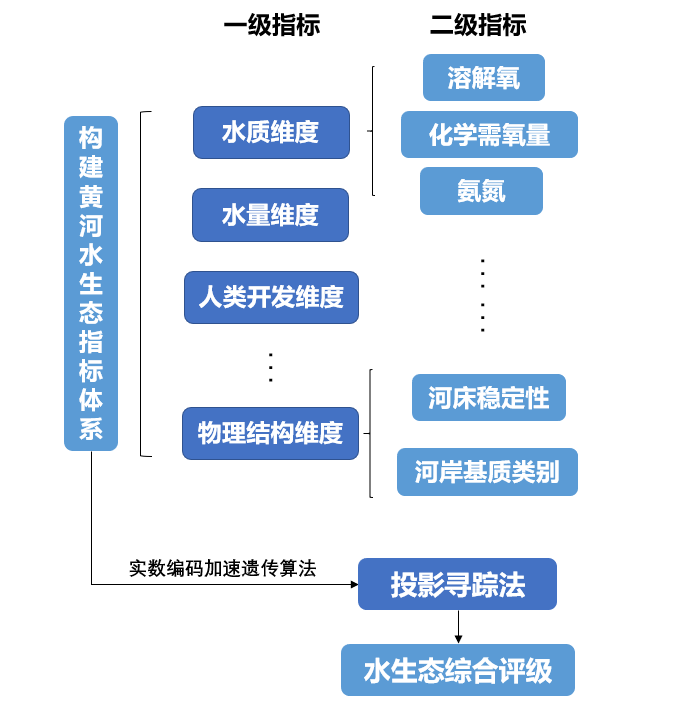
\includegraphics[width=.8\textwidth]{问题三思路图.png}
	\caption{问题三思路图}
	\label{变化趋势}
\end{figure}

\subsection{补充数据}


水生态的评价比较复杂,需要通过查阅相关文献以获取更多例如
径流变化率等水文数据。收集到的数据如表\ref{数据}所示。分级指标如表\ref{分级}所示。
% Table generated by Excel2LaTeX from sheet 'Sheet1'
\begin{table}[H]
	\centering
	\caption{数据及来源}\scriptsize
	  \begin{tabular}{p{6.8em}m{1cm}<{\centering}m{1cm}<{\centering}m{1cm}<{\centering}m{1cm}<{\centering}m{1cm}<{\centering}m{1cm}<{\centering}m{0.8cm}<{\centering}m{1cm}<{\centering}p{11.6em}}\toprule[1.5pt]
	  指标名称 & \multicolumn{1}{p{3.2em}}{1月} & \multicolumn{1}{p{3.2em}}{2月} & \multicolumn{1}{p{3.2em}}{3月} & \multicolumn{1}{p{3.2em}}{4月} & \multicolumn{1}{p{3.2em}}{5月} & \multicolumn{1}{p{3.2em}}{6月} & \multicolumn{1}{p{3.2em}}{7月} & \multicolumn{1}{p{3.2em}}{8月} & 数据来源 \\\hline
	  人均水资源占有量 & \multicolumn{8}{c}{960}                       & 《2018年宁夏水资源公报》 \\\hline
	  径流变化率 & 0.56 & 0.47 & 0.51 & 0.68 & 1.09 & 1.15 & 1.8 & 1.76 & 《黄河上游宁蒙河段径流特征分析及预测》 \\\hline
	  含沙量变化率 & \multicolumn{8}{c}{0.2145}                    & \multirow{2}[0]{*}{《中国河流泥沙公报》} \\
	  生态流量保证程度 & \multicolumn{3}{c}{0.3214} & \multicolumn{5}{c}{0.4125}  & \multicolumn{1}{c}{} \\\hline
	  万元生产总值用水量 & \multicolumn{8}{c}{179}                       & \multirow{3}[0]{*}{《2018年宁夏水资源公报》} \\
	  万元工业增加值用水量 & \multicolumn{8}{c}{91}                        & \multicolumn{1}{c}{} \\
	  农业灌溉水利用系数 & \multicolumn{8}{c}{0.42}                      & \multicolumn{1}{c}{} \\\hline
	  水资源开发利用率/\% & \multicolumn{8}{c}{48.4}                      & 《宁夏地下水资源分布特征及开发利用现状研究》 \\\hline
	  河床稳定性 & \multicolumn{8}{c}{砂卵河床}                & 《黄河上游宁蒙河段径流特征分析及预测》 \\\hline
	  河岸基质类别 & \multicolumn{8}{c}{非黏土河岸}               & 《中国河流泥沙公报》 \\\hline
	  河流平均比降/\% & \multicolumn{8}{c}{11.6}                      & 《黄河上游宁蒙河段径流特征分析及预测》 \\ \bottomrule[1.5pt]
	  \end{tabular}%
	\label{数据}%
  \end{table}%

\begin{table}[H]
	\centering
	\caption{分级标准}\scriptsize
    \begin{tabular}{p{4.19em}p{10.44em}cccccc}\toprule[1.5pt]
		指标类别 & 指标名称 & \multicolumn{1}{p{4.94em}}{Ⅰ类} & \multicolumn{1}{p{4.94em}}{Ⅱ类} & \multicolumn{1}{p{4.94em}}{Ⅲ类} & \multicolumn{1}{p{4.94em}}{Ⅳ类} & \multicolumn{1}{p{4.94em}}{Ⅴ类} & \multicolumn{1}{p{8.065em}}{数据来源} \\ \hline
		水量维度 & 人均水资源占有量 & 3500 & 2200 & 1700 & 1000 & 500 & \multicolumn{1}{p{8.065em}}{《黄河流域水资源评价研究》} \\ \hline
		水文维度 & 径流变化率 & 100 & 95  & 90  & 80  & 65  & \multicolumn{1}{p{8.065em}}{《黄河内蒙古段河流健康评价》} \\ \hline
		\multicolumn{1}{c}{} & 含沙量变化率 & 0.05 & 0.15 & 0.2 & 0.25 & 0.4 & \multicolumn{1}{c}{\multirow{2}[0]{*}{《地表水环境质量标准》}} \\ 
		\multicolumn{1}{c}{} & 生态流量保证程度 & 0.5 & 0.4 & 0.3 & 0.1 & 0   &  \\\hline
		人类开发维度 & 万元生产总值用水量 & 24  & 60  & 140 & 220 & 500 & \multicolumn{1}{c}{\multirow{7}[0]{*}{《黄河流域水资源评价研究》}} \\
		\multicolumn{1}{c}{} & 万元工业增加值用水量 & 0   & 15  & 50  & 100 & 300 &  \\
		\multicolumn{1}{c}{} & 农业灌溉水利用系数 & 0.6 & 0.5 & 0.4 & 0.3 & 0   &  \\
		\multicolumn{1}{c}{} & 水资源开发利用率/\% & 10  & 20  & 40  & 60  & 100 &  \\
		物理结构维度 & 河床稳定性 & 1   & 2   & 3   & 4   & 5   &  \\
		\multicolumn{1}{c}{} & 河岸基质类别 & \multicolumn{1}{p{4.94em}}{基岩} & \multicolumn{1}{p{4.94em}}{基岩} & \multicolumn{1}{p{4.94em}}{岩土河岸} & \multicolumn{1}{p{4.94em}}{黏土河岸} & \multicolumn{1}{p{4.94em}}{非黏土河岸} &  \\
		水流维度 & 河流平均比降/\% & 10  & 20  & 30  & 40  & 50  &  \\\bottomrule[1.5pt]
		\end{tabular}%
	\label{分级}%
\end{table}%

\subsection{基于加速遗传算法的投影寻踪评价模型}
投影寻踪(PP)属于直接由样本数据驱动的探索性数据分析方法,可以将高维数据通过
组合投影到低维空间,通过寻找最优投影函数来使得投影能反映高维数据的结构或者特征。
~\\
\textbf{1)评价指标归一化}

设样本集为$x^*_{(i,j)},i=1,2,...,n\quad j=1,2,...,p$其中$x_{(i,j)}$为第i个样本
第j个指标值。为消除各指标的量纲和统一化各指标的变化范围,可采用下式进行极值进行
归一化处理:

\begin{equation}
	\label{2}
	\begin{split}
		x_{(x,j)}=\frac{x^*_{(i,j)}-Ex(j)}{Sx(j)},
	\end{split}
\end{equation}
式中,$Ex(j)$、$Sx(j)$分别为第j个指标值的均值和标准差。

~\\
\textbf{2)构造投影指标函数}

将p维数据$\{x_{(i,j)}|j=1,2,...,p\}$以$a=(a_1,a_2,...,a_p)$方向投影为一维值$Z_i$
\begin{equation}
	\label{2}
	\begin{split}
		Z_i=\sum_{j=1}^pa_jx_{(i,j)},
	\end{split}
\end{equation}
式中$a$为单位长度向量。

在综合投影值时,要求投影值$Z_i$散布特征为:1、投影值$Z_i$尽可能多
的提取到$\{x_{(i,j)}\}$中的变异信息,即$Z_i$的标准差$S_z$达到尽可能大,同时要求$Z_i$与
已知标准等级$y_i$的相关系数的绝对值$\lvert R_{zy} \rvert$达到尽可能大。为此,投影指标函数
可构造为

\begin{equation}
	\label{2}
	\begin{split}
		Q(a)=S_z\lvert R_{zy} \rvert,
	\end{split}
\end{equation}
式中,$S_z$为投影值$R_{zy}$的标准差。式中$S_z$、$R_{zy}$分别为

\begin{equation}
	\label{2}
	\begin{split}
		Q(a)=S_z\lvert R_{zy} \rvert,
	\end{split}
\end{equation}
式中,$S_z$和$R_{zy}$分别为

\begin{equation}
	\label{2}
	\begin{split}
		&S_z=[\frac{\sum_{i=1}^n(Z_i-EZ)^2}{n-1}]^{0.5},\\
		&R_z=\frac{\sum_{i=1}^n(Z_i-EZ)(y_i-Ey)}{[\sum_{i=1}^n(Z_i-EZ)^2\sum_{i=1}^n(y_i-Ey)^2]^{0.5}}.
	\end{split}
\end{equation}

~\\
\textbf{3)优化投影指标函数}
当各个指标值的样本集给定时间,投影函数值$Q(a)$只随着投影方向$a$的变化而变化。不同的投影方向反映不同的数据
特征,最佳投影方向就是最大可能暴露高纬度数据某类特征的投影方向。可通过求解投影指标函数最大化问题
来估计最佳投影方向:

\begin{equation}
	\label{2}
	\begin{split}
	&max Q(a)=S_z\lvert R_{zy} \rvert\\,
	&s.t. \sum_{j=1}^pa^2(j)=1.
	\end{split}
\end{equation}
~\\
\textbf{4)建立投影寻踪等级评价模型}

将步骤三求得的最佳投影方向的估计$a^*$代入投影值公式,得第i个样本投影值的计算值$Z^*_i$,
根据$Z^*_i-y_i$的散点图建立相应的等级评价模型。$Z^*_i$与$y^(i)$之间一般呈现单调非降关系,
当$Z^*_i$值超过某门限值就会判定最高等级,当指标值低于另门限值就会判定为最低等级,当$Z^*_i$
介于这两点中间时则为中等等级,可以用逻辑斯蒂曲线来描述:

\begin{figure}[H]
	\centering
	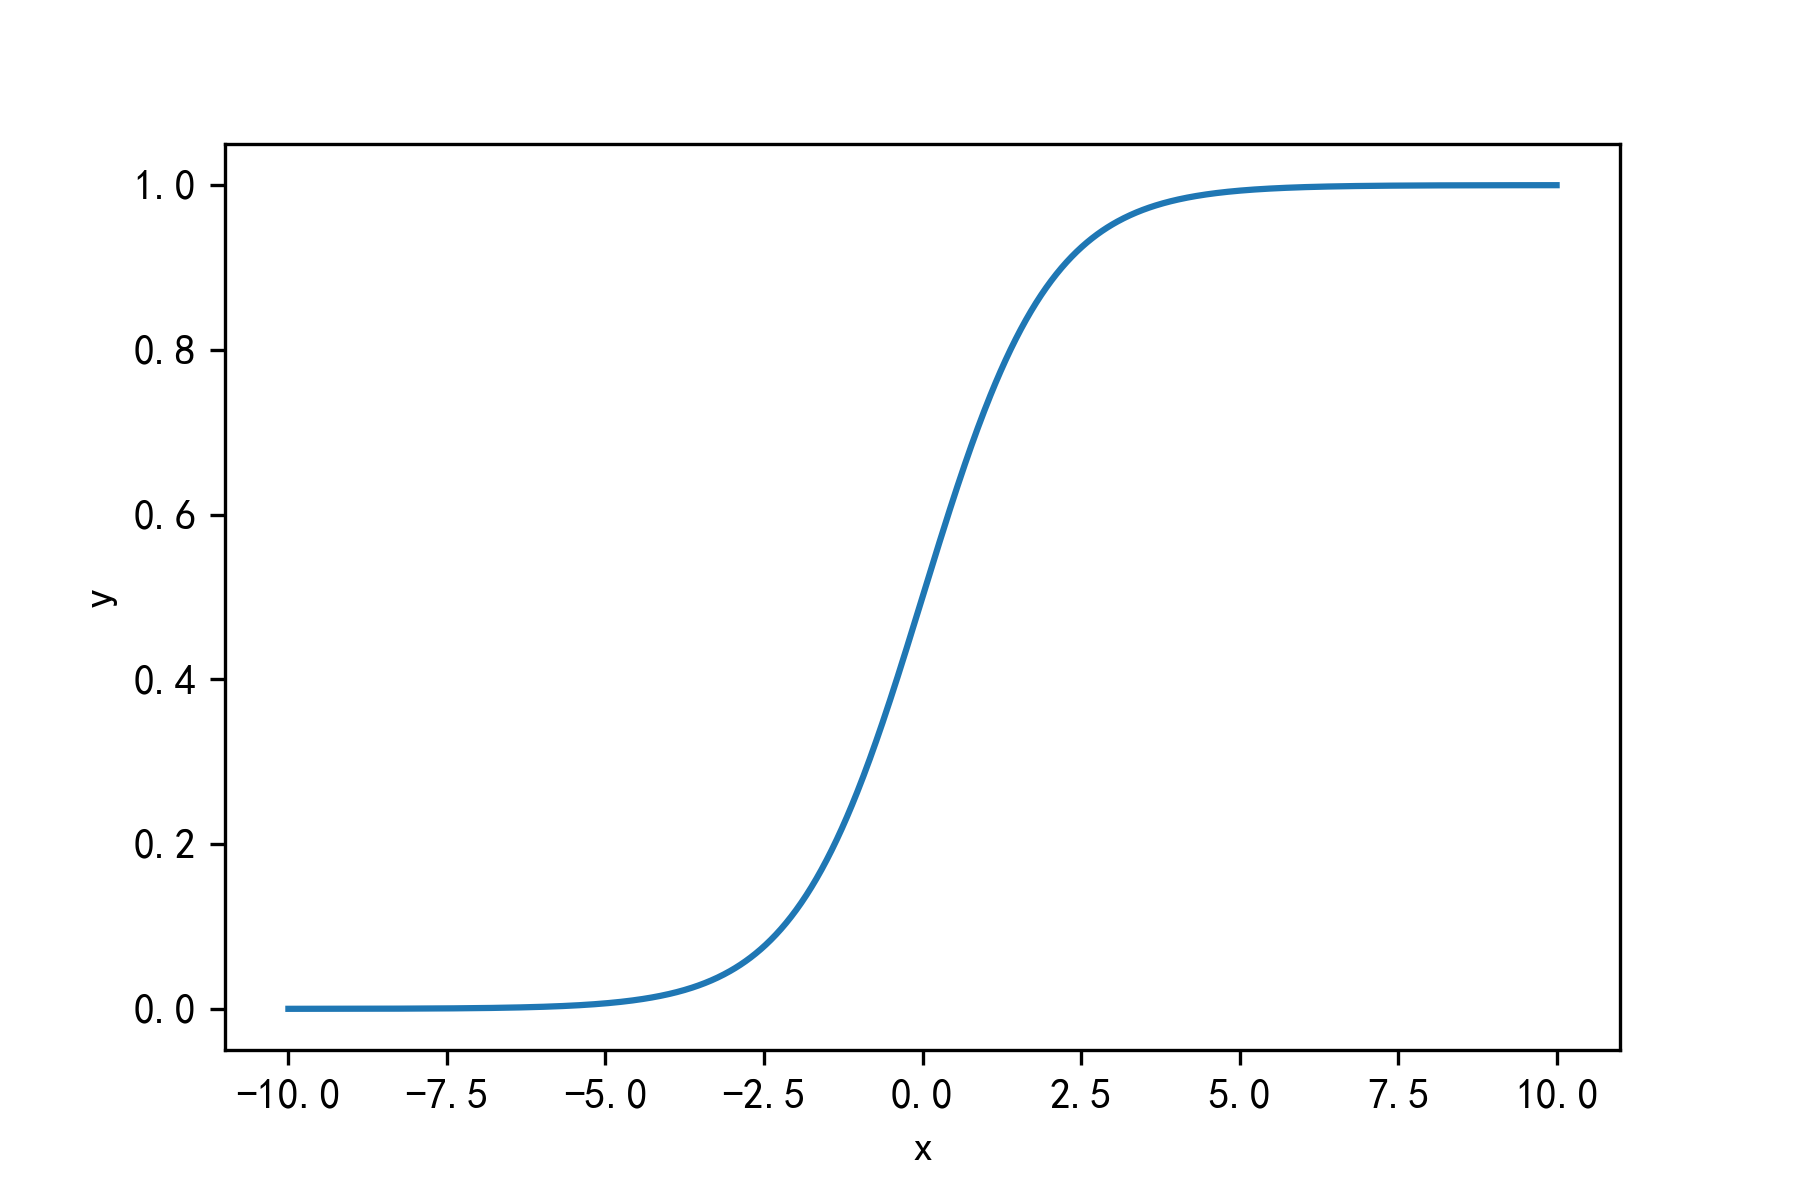
\includegraphics[width=.5\textwidth]{逻辑斯蒂.png}
	\caption{逻辑斯蒂曲线示意图}
	\label{变化趋势2}
\end{figure}

\begin{equation}
	\label{2}
	\begin{split}
    y_i^*=\frac{N}{1+e^{c_1-c_2Z^*_i}},
	\end{split}
\end{equation}
式中$y_i^*$为第i个样本等级的计算值;模型参数$c_1$、$c_2$分别为积分常数和增长率,可通过求解
如下优化问题来确定:

\begin{equation}
	\label{2}
	\begin{split}
    min F(c_1,c_2)=\sum_{i=1}^n(y_i^*-y_i)^2.
	\end{split}
\end{equation}

\subsection{加速遗传(AGA)算法求解}

加速遗传(AGA)算法对于普通遗传算法的改进:

1)控制参数设置:每次加速循环中的AGA只循环两次SGA的进化迭代。

2)p个变量、加数循环q次,优秀个体包围最优点的概率为$(1-0.5^{2s})^{pq}$。

以下是AGA求解伪代码:

\begin{algorithm}
	\caption{Function AGAPPGE(x)}
	\LinesNumbered
	StandardScaler(x)
	\tcc{归一化:为消除量纲与指标值的变换范围,对数据进行归一化}
	\textbf{Initialize}
	\tcc{初始话:初始化种群}
	iteration = 1;
	\textbf{Repeat}
	\For{$i \in [1,N]$}{
		ComputeFeasibility($x_i$) \tcc{计算适应度}
		Sort($x_i$) \tcc{按照适应度进行排序}
		Evaluate($x_i$) \tcc{计算基于序的评价函数}
		Select($x_i$) \tcc{选择操作}
		Mutate($x_i$) \tcc{变异操作}
		Merge($x_i$) \tcc{合并交叉部分和剩余部分}
	}
	iteration $\leftarrow$ iteration$+1$; {\mbox{进入下一次迭代}} \newline
	until \mbox{达到迭代次数。}
\end{algorithm}
~\\

通过matlab求解,得到一到八月每个节点的水生态评分如表\ref{得分},表中分数越低则说明该月该节点
的水生态越恶劣。

% Table generated by Excel2LaTeX from sheet 'Sheet2'
\begin{table}[htbp]
	\centering
	\caption{各月份各断面水质细分表}
	  \begin{tabular}{ccccccccc}\toprule[1.5pt]
        & 1月  & 2月  & 3月  & 4月  & 5月  & 6月  & 7月  & 8月 \\ \hline
    A   & 2.231876 & 3.051511 & 2.474963 & 2.332324 & 2.801374 & 2.508442 & \textbackslash{} & \textbackslash{} \\
    B   & 2.137685 & 2.330664 & 2.766444 & 2.019016 & 2.478643 & 2.005526 & 2.797785 & 2.796999 \\
    C   & 2.329781 & 2.933338 & 2.799032 & 2.54852 & 2.493417 & 2.345483 & 2.818519 & 2.938506 \\
    D   & 3.574317 & 3.452619 & 2.802116 & 2.943436 & 2.763737 & 2.921222 & 2.839983 & 2.880777 \\
    E   & 3.410205 & 3.307502 & 3.171557 & 2.795494 & 2.499318 & 2.351724 & 2.183836 & 3.085028 \\ \bottomrule[1.5pt]
    \end{tabular}%
	\label{得分}%
  \end{table}%

  \begin{figure}[H]
	\centering
	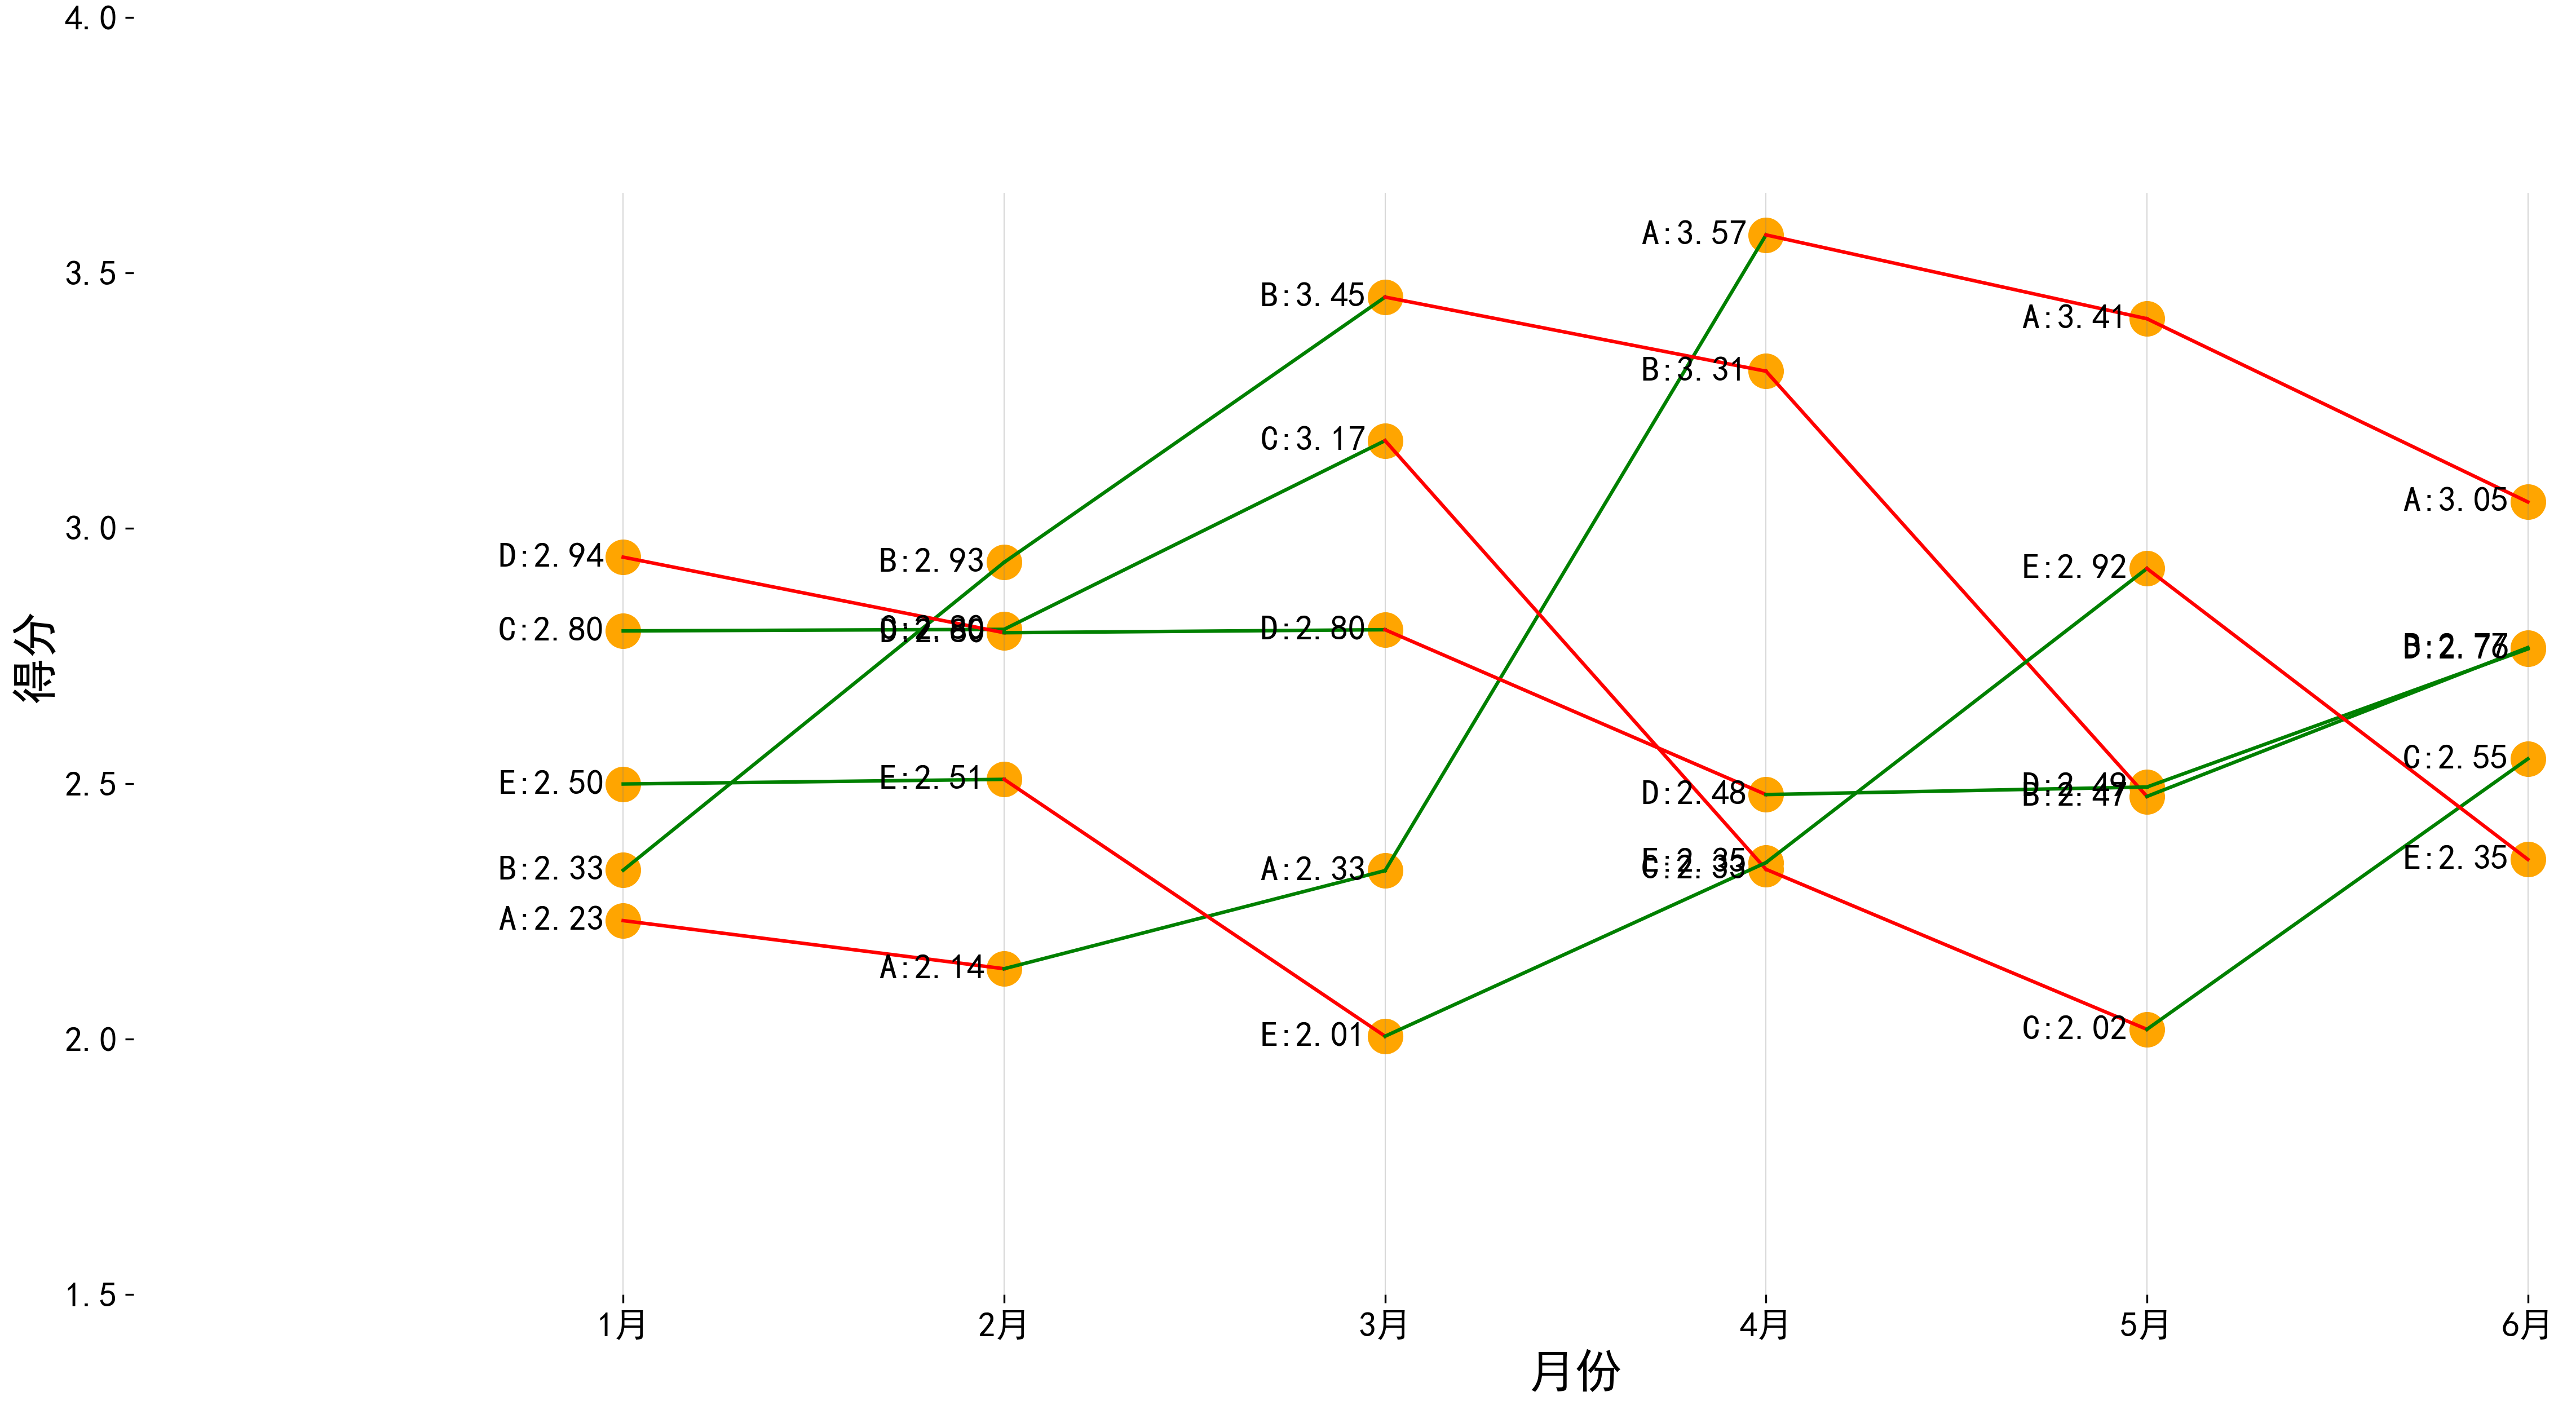
\includegraphics[width=.9\textwidth]{得分变化1.png}
	\caption{各个断面1到6月得分趋势图}
	\label{变化趋势1}
\end{figure}


\begin{figure}[H]
	\centering
	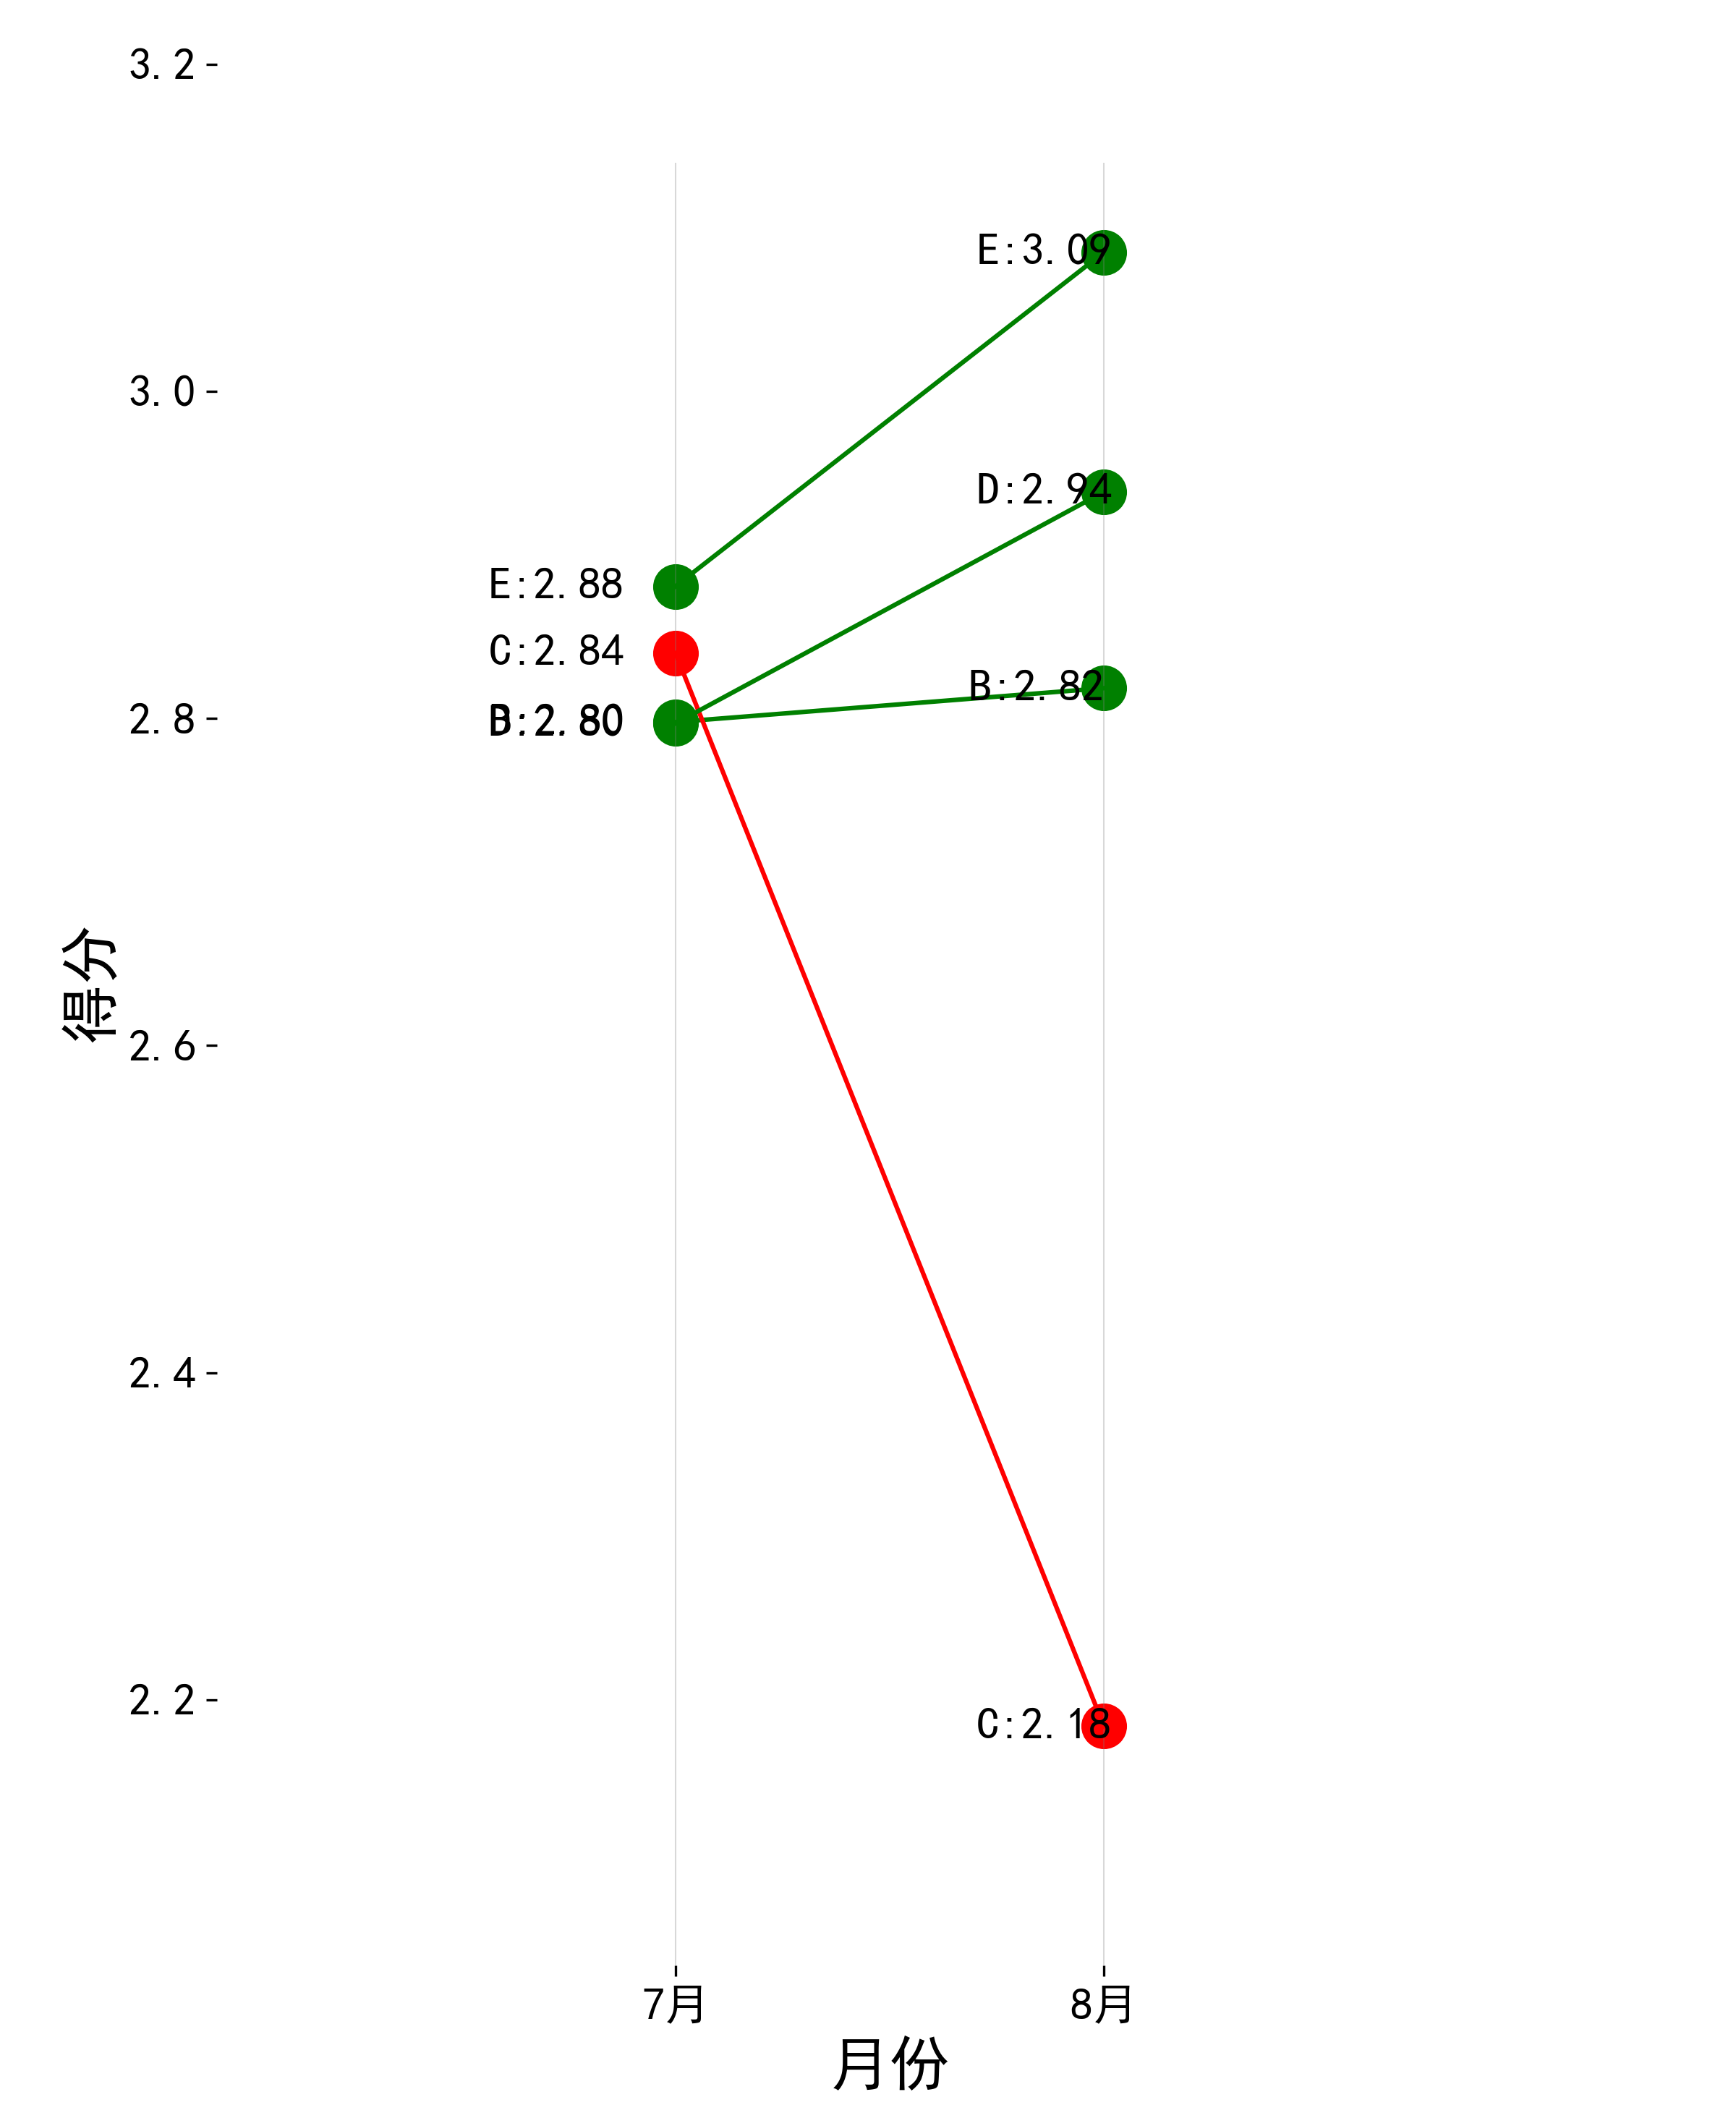
\includegraphics[width=.5\textwidth]{得分变化2.png}
	\caption{各个断面7到8月得分趋势图}
	\label{变化趋势2}
\end{figure}

图\ref{变化趋势1}、图\ref{变化趋势2}为枯水期和丰水期各个断面随着时间变化的趋势折线图。每个断面的评分为利用投影寻踪法求出的
水质评分。通过评分可以观察每个截面水质在时间上的变化。


  在计算出各断面的水生态得分后,为更客观的反映相应水质的优劣,本文拟引入各指标
  的分级标准(具体分级阈值见表\ref{分级}分级标准),并将每一级的指标阈值代入到
  上述的投影寻踪评价模型中,得到水生态综合等级划分阈值,见表\ref{阈值}:

  % Table generated by Excel2LaTeX from sheet 'Sheet1'
\begin{table}[H]
	\centering
	\caption{分类等级评分}
	  \begin{tabular}{cccccc} \toprule[1.5pt]
	 分类等级& I类  & II类 & III类 & IV类 & V类 \\ \hline
	  评分&4.045987 & 3.327785 & 2.436266 & 1.232433 & 0.299109 \\ \bottomrule[1.5pt]
	  \end{tabular}%
	\label{阈值}%
  \end{table}%
  
将表6各月份各断面水质细分表的数据分别代入至表7分类等级评分中,最终得到各断面的水生态
等级。需要说明,其中Ⅰ类表示水生态健康,Ⅴ类表示水生态严重不健康。

  \begin{table}[H]
	\centering
	\caption{各月份各断面水质细分表}
	  \begin{tabular}{ccccccccc}\toprule[1.5pt]
        & 1月  & 2月  & 3月  & 4月  & 5月  & 6月  & 7月  & 8月 \\ \hline
		A   & IV  & III & III & IV  & III & III & \textbackslash{} & \textbackslash{} \\
		B   & IV  & IV  & III & IV  & III & IV  & III & III \\
		C   & IV  & III & III & III & III & IV  & III & III \\
		D   & II  & II  & III & III & III & III & III & III \\
		E   & II  & III & III & III & III & IV  & IV  & III \\ \bottomrule[1.5pt]
    \end{tabular}%
	\label{得分}%
  \end{table}%
	



\subsection{结果分析}
	
从整体分析,存在较多的生态整体情况不达标。
从时间上看枯水期的生态情况不容乐观,一月和二月的评分较低,究其原因可能为黄河冰冻期,河流
流速缓慢并且冬季取暖导致污水排放增加,而三、四月份河流解冻流速和流量都增加所以导致污染物
浓度下降,评分增加。四五月份为枯水期界面流量的下降导致了浓度的增加。从数据上来看,
污染物浓度变化影响的水质指标的变化对水生态评分的影响最大。


综上,基于相关资料,本文判断此评价模型能较为客观的反映出黄河宁夏段的水生态情况。同时本文认为
维护水生态最快速的方式就是改善水质情况,减少水污染。从产业的角度来说,如今整个黄河流域产业体
系上偏重,煤炭、有色占了比较大的比例,资源性重度污染在黄河流域上游出现较多,并且目前仍有大量企业在
黄河沿岸随意排放污水,因此如何监管企业的污水处理情况十分重要,有关部门需要加大监管力度。

\section{模型总结与评价}


\subsection{模型优点}
1.模糊综合评价从整体水质的角度进行了描述,与国家标准中规定的以最劣指标划分等级的方法相结合,使得评价结果
更为全面。

2.运用了投影寻踪法对水生态情况进行分析,能够获得客观、科学的评价,且评分为连续的数值,比等级评价的结果更
为细致。

3.通过经验正交函数分解法得到了水质指标的时空模态,并从时间和空间两个维度进行分析。除了能够分析单一指标
的时空趋势,还能够得到任意两断面之间变化的关联性。

\subsection{模型缺点}
1.由于附件未标明数据来源的年份和具体经纬度,故在第三问补充数据时仅能保证数据皆为同一个月份,导致评价结果
存在一定偏差。

\subsection{模型改进}
目前,对于水污染的动力学模拟为当前的研究热点,国内外的诸多学者也提出了诸如WASP、StreeterPhelps、QUAL等
水质模型。由于附件中缺少断面具体位置的描述,故未能实施。若将来能获取更为全面的数据,可基于污染物扩散机理,
对污染源回溯、污染物降解过程进一步模拟分析。

\clearpage

\addcontentsline{toc}{section}{参考文献}



	%参考文献
\begin{thebibliography}{9}%宽度9
		\bibitem{bib:one} 景朝霞,夏军,张翔,等.汉江中下游干流水质状况时空分布特征及变化规律[J].环境科学研究,2019,32(01):104-115.
		\bibitem{bib:two} 彭亚辉,周科平,蒋俊伟.湘江流域长株潭段水污染负荷时空分布规律及成因[J].中国农业大学学报,2018,23(09):108-116.
		\bibitem{bib:three}贺磊.基于熵权法-正态云模型的辽宁省水生态承载力评价[J].水资源开发与管理,2020(07):16-22.
		\bibitem{bib:four} 隋欣,齐晔.基于生态系统健康的生态承载力调控模式研究[J].应用基础与工程科学学报,2006(04):479-487.
		\bibitem{bib:five}阿提卡木·阿布来提.不同水质评价方法在喀什地区地下水水质评价中的适用性分析[J].地下水,2020,42(04):49-50+80.
		\bibitem{bib:five}陈明霞,熊贵耀,张佳鹏,等.湘江流域水质综合评价及其时空演变分析[J].环境工程,2019,37(10):83-90+104.
		\bibitem{bib:five}李琪,赵志怀.基于投影寻踪与内梅罗指数组合模型的地下水水质评价[J].水电能源科学,2019,37(11):70-73.

\end{thebibliography}

	\clearpage

	\appendix %%附录



\section{代码}
\subsection{ python 源程序}
ss\begin{lstlisting}[language=python]
	def compute_gbstd(df, gbdata):
    roma=['Ⅰ类','Ⅱ类','Ⅲ类','Ⅳ类','Ⅴ类']
    ms = np.zeros((1, len(df.index)))

    for idx, col in enumerate(df.index):
        if col not in ['溶解氧']:
            if df[col] < np.float64(gbdata[gbdata['feature'] == col][roma[0]]):
                ms[0, idx] = 1
            elif df[col] > np.float64(gbdata[gbdata['feature'] == col][roma[-1]]):
                ms[0, idx] = 5
            else:
                for i in range(5):
                    if df[col] < np.float64(gbdata[gbdata['feature'] == col][roma[i]]):
                        ms[0, idx] = i+1
                        break
        else:
            if df[col] > np.float64(gbdata[gbdata['feature'] == col][roma[0]]):
                ms[0, idx] = 1
            elif df[col] < np.float64(gbdata[gbdata['feature'] == col][roma[-1]]):
                ms[0, idx] = 5
            else:
                for i in range(5):
                    if df[col] > np.float64(gbdata[gbdata['feature'] == col][roma[i]]):
                        ms[0, idx] = i+1
                        break
    return max(max(ms))
\end{lstlisting}

	\subsection{粒子群算法 matlab 源程序}
	\begin{lstlisting}[language=matlab]
	%% Particle Swarm Optimization
	clc
	clear
	global dots
	global dismat
	global path_var
	load dots
	load('../dismat1')
	load path_var
	%% Problem Statement
	Npar = 2;
	FN = 'BenchmarkFunction';
	FunNumber = 6;
	VarLow = -5;
	VarHigh = 5;
	
	%% Parameters
	C1 = 1.5;
	C2 = 4-C1;
	Inertia = .3;
	DampRatio = .95;
	ParticleSize = 10;
	MaxIter = 200;
	
	GlobalBest = 0;
	GlobalBestCost = 10000;
	
	%% Initialization
	GB = [];
	
	for ii = 1:ParticleSize
		Particle{ii}.Position = rand(1,Npar) * (VarHigh - VarLow) + VarLow;
		Particle{ii}.Position = fix_coordinate(Particle{ii}.Position);
		Particle{ii}.Cost = feval(FN,Particle{ii}.Position);
		Particle{ii}.Velocity = rand(1,Npar);
		Particle{ii}.LocalBest = Particle{ii}.Position;
		Particle{ii}.LocalBestCost = Particle{ii}.Cost;
		if Particle{ii}.Cost < GlobalBestCost
			GlobalBest = Particle{ii}.Position;
			GlobalBestCost = Particle{ii}.Cost;
		end
	end
	
	%% Main Loop
	for jj = 1:MaxIter
		for ii = 1:ParticleSize
			Inertia = Inertia * DampRatio;
			Particle{ii}.Velocity = rand * Inertia * Particle{ii}.Velocity + C1 * rand * (Particle{ii}.LocalBest - Particle{ii}.Position) +  C2 * rand * (GlobalBest - Particle{ii}.Position);
			Particle{ii}.Position = Particle{ii}.Position + Particle{ii}.Velocity;
	
			Particle{ii}.Position(Particle{ii}.Position > VarHigh) = VarHigh;
			Particle{ii}.Position(Particle{ii}.Position < VarLow) = VarLow;
			Particle{ii}.Position = fix_coordinate1(Particle{ii}.Position);
			Particle{ii}.Cost = feval(FN,Particle{ii}.Position);
			if Particle{ii}.Cost < Particle{ii}.LocalBestCost
				Particle{ii}.LocalBest = Particle{ii}.Position;
				Particle{ii}.LocalBestCost = Particle{ii}.Cost;
	
				if Particle{ii}.Cost < GlobalBestCost
					Particle{ii}.Cost
					GlobalBest = Particle{ii}.Position;
					GlobalBestCost = Particle{ii}.Cost;
				end
			end
		end
		GB = [GB GlobalBestCost];
	end
	
	% %% Function Plot
	% x = -10:.05:10;
	% y = -10:.05:10;
	% [X,Y] = meshgrid(x,y);
	% Z = 60 + X.^2 + Y.^2 - 30*(cos(20* X) + cos(20*Y));
	% surf(X,Y,Z)
	%%
	plot(GB,'LineWidth',1.5)
	GlobalBest
	GlobalBestCost
	
\end{lstlisting}

	\subsection{fix coordinate matlab 源程序}
	\begin{lstlisting}[language=matlab]
	
	function x = fix_coordinate(x)
global dots
for i = 1:size(x,1)
    if x(i,2) < -4
        x(i,2) = -4;
    end
    if x(i,1) > -1 && x(i,1) < 0 && x(i,2) > 3
        x(i,2) = 3;
    end
    ra = rand;
    if x(i,1) > -3 && x(i,1) < -1 && x(i,2) > 1 && x(i,2) < 3
        if ra < 0.25
            x(i,1)=-3;
        elseif ra >= 0.25 && ra < 0.5
            x(i,1)=-1;
        elseif ra >=0.5 && ra < 0.75
            x(i,2)=1;
        else
            x(i,2)=3;
        end
    end
    if x(i,1) >= 0 && x(i,1) <=5 && x(i,2) > 4
        x(i,2) = 4;
    end
    if rand > 0.5
        x(i,2) = round(x(i,2));
        x1 = floor(x(i,1));
        x2 = ceil(x(i,1));
        y1 = x(i,2);
        y2 = x(i,2);
    else
        x(i,1) = round(x(i,1));
        x1 = x(i,1);
        x2 = x(i,1);
        y1 = floor(x(i,2));
        y2 = ceil(x(i,2));
    end
    % 存在dot1和dot2重合的情况
    dot1 = find(dots(:,1)==x1 & dots(:,2)==y1);
    dot2 = find(dots(:,2)==x2 & dots(:,2)==y2);
    if isempty(dot1) && isempty(dot2)
        ra = rand;
        if ra <0.25
            x(i,1) = x(i,1)+1;
        elseif ra >=0.25 && ra < 0.5
            x(i,1) = x(i,1)-1;
        elseif ra >= 0.5 && ra < 0.75
            x(i,2) = x(i,2)+1;
        else
            x(i,2) = x(i,2)-1;
        end
    elseif isempty(dot1)
        x(i,1) = x2;
        x(i,2) = y2;
    elseif isempty(dot2)
        x(i,1) = x1;
        x(i,2) = y1;
    end
end
\end{lstlisting}
\end{spacing}
\end{document}